% !TeX document-id = {9cf4a256-69f9-4753-af64-0a80ece20722}
% !TeX encoding = UTF-8
% !TeX TXS-program:compile = latexmk.exe -silent -synctex=1 %
% !TeX TXS-program:view = txs:///view-pdf-internal --embedded build/main.pdf
\documentclass[a4paper,fleqn]{cas-sc}
% If the frontmatter runs over more than one page
% use the longmktitle option.

%\documentclass[a4paper,fleqn,longmktitle]{cas-sc}

\usepackage[numbers]{natbib}
% \usepackage[authoryear]{natbib}
% \usepackage[authoryear,longnamesfirst]{natbib}

\usepackage{bm}
\usepackage{amsmath,amssymb,amsfonts}
\usepackage{graphicx}
\graphicspath{{figures/}}
\usepackage{float}
\usepackage{placeins}
%\usepackage{xeCJK}
\usepackage{booktabs}
\usepackage{multirow}
\usepackage{array}
\usepackage{pifont}
\usepackage{adjustbox}
\usepackage{caption}
\usepackage{subcaption}
\usepackage{tabularx}
\usepackage{rotating}
\usepackage{makecell}
\usepackage{threeparttable}
\usepackage{enumitem}
\captionsetup{
	font=small,
	labelfont=bf,
	labelsep=period,
	skip=4pt
}

\setlength{\textfloatsep}{8pt plus 2pt minus 2pt}
\setlength{\floatsep}{6pt plus 2pt minus 2pt}
\setlength{\intextsep}{6pt plus 2pt minus 2pt}
\renewcommand{\arraystretch}{1.08}

%%% Author macros
\def\tsc#1{\csdef{#1}{\textsc{\lowercase{#1}}\xspace}}
\tsc{WGM}
\tsc{QE}
%%%
% Uncomment and use as if needed
%\newtheorem{theorem}{Theorem}
%\newtheorem{lemma}[theorem]{Lemma}
%\newdefinition{rmk}{Remark}
%\newproof{pf}{Proof}
%\newproof{pot}{Proof of Theorem \ref{thm}}

 \begin{document}
	\let\WriteBookmarks\relax
	\renewcommand{\floatpagefraction}{0.82}
	\renewcommand{\textfraction}{0.10}
	\renewcommand{\topfraction}{0.90}
	\renewcommand{\dbltopfraction}{0.90}
	\setcounter{topnumber}{3}
	\setcounter{dbltopnumber}{2}
	
	% Short title
	\shorttitle{}
	
	% Short author
	\shortauthors{Wang et~al.}
	
	% Main title of the paper
	\title[mode=title]{EGCS-Net: An Explicit Geometry-Conditioned Segmentation Network for Retinal Vessel Segmentation}
	
	% Title footnote mark
	% eg: \tnotemark[1]
	\tnotemark[1]
	
	\tnotetext[1]{Code and data is available at \url{https://github.com/YF-W}}
	
	
	\author[1]{Yuefei Wang}[orcid=0000-0003-3032-1852]
	\cormark[1]
	\cortext[1]{Corresponding author}
	\ead{wangyuefei@cdu.edu.cn}
	
	\author[2]{Junji Chen}
	
	\author[2,3]{Pedro Mestre}

	\author[1]{Guanwen Wang}

	\author[1]{Tianyu He}

	\author[1]{Liangyan Zhao}
	
	\author[1]{Haikun Tan}

	\affiliation[1]{organization={College of Computer Science},
		addressline={Chengdu University},
		city={Chengdu},
		postcode={610106},
		state={Sichuan},
		country={China}}
	
	\affiliation[2]{organization={Stirling College},
		addressline={Chengdu University},
		city={Chengdu},
		postcode={610106},
		state={Sichuan},
		country={China}}
	
	\affiliation[3]{organization={Algoritmi Research Center},
		addressline={University of Minho},
		country={Portugal}}

	
	% Here goes the abstract
	\begin{abstract}
	Retinal vessel segmentation requires the recovery of thin, continuous, and branching structures across large variations in vessel scale and image contrast. Existing encoder-decoder, attention-based, and Transformer-based methods mainly perform dense prediction on Cartesian grids, leaving the spatial organization of vessels to be learned implicitly. Consequently, an explicit geometric reference, spatially varying directional organization, and selective high-resolution detail transfer remain insufficiently coupled. We therefore propose EGCS-Net, the Explicit Geometry-Conditioned Segmentation Network, which formulates retinal vessel segmentation as geometry-conditioned structure recovery. In its dual-branch coarse-to-fine framework, a structure-prior branch guides a detail-refinement branch through cascaded and same-scale feature injection. Reference Center Elicitation (RCE) estimates a learned center state for geometric organization. Sector Geometry Conditioning (SGC) uses this state to model angular and radial relationships with dual-ring soft sectors. Connectivity-Preserving Skip Purification (CSP) filters the final high-resolution skip information before reconstruction. On AV-WIDE, ARIA, DRIVE, CHASEDB1, and STARE, EGCS-Net achieves the highest Dice and IoU among the compared methods on each dataset, with five-dataset averages of 56.94\% and 41.49\%, respectively. Integrating RCE, SGC, and CSP into U-Net, UNet++, and TransUNet also improves Dice and IoU for every evaluated backbone-dataset combination. These results support the use of explicit geometric conditioning to coordinate global vessel organization with controlled detail reconstruction in the evaluated settings.
	\end{abstract}
	
	% Use if graphical abstract is present
	%\begin{graphicalabstract}
	%\includegraphics{}
	%\end{graphicalabstract}
	
	% Research highlights
	% \begin{highlights}
		% \item
		% \item
		% \item
		% \end{highlights}
	
	% Keywords
	% Each keyword is separated by \sep

	\begin{keywords}
	Retinal vessel segmentation \sep geometric priors \sep structural conditioning \sep sector geometry \sep skip-connection refinement
	\end{keywords}

	\maketitle
	
	% Main text
	\section{Introduction}

Retinal vessel segmentation aims to recover a connected vascular tree rather than classify vessel pixels independently.
Accurate vessel maps support quantitative assessment of vascular caliber, branching, and topology and contribute to the analysis of diabetic retinopathy, hypertensive retinopathy, glaucoma, and other conditions\cite{fraz2012blood,patton2006retinal}.
This task remains difficult because retinal vessels include wide trunks and very thin branches, change direction throughout the field of view, and may have weak contrast against nonuniform backgrounds.
A useful segmentation model must therefore preserve continuity over long distances and recover fine detail without converting background texture into false vessel responses.

Supervised U-shaped networks, including U-Net, UNet++, and nnU-Net, provide strong baselines for medical image segmentation\cite{ronneberger2015u,zhou2018unet++,isensee2021nnu}.
Context aggregation and Transformer-based interaction further extend the ability of these networks to combine local detail with global information\cite{chen2024transunet,cao2022swin}.
These approaches improve generic feature representation, but they generally retain pixelwise dense prediction on Cartesian grids.
The spatial organization of the vascular tree is therefore learned largely from appearance and context rather than represented as an explicit condition.
This implicit treatment can leave thin branches, weak vessel responses, and complex bifurcations vulnerable to discontinuity, directional confusion, and background activation.

The geometric contrast that motivates the proposed method is illustrated in Figure~\ref{fig:yingyan3}.

\begin{figure}[pos=!htbp]
    \centering
    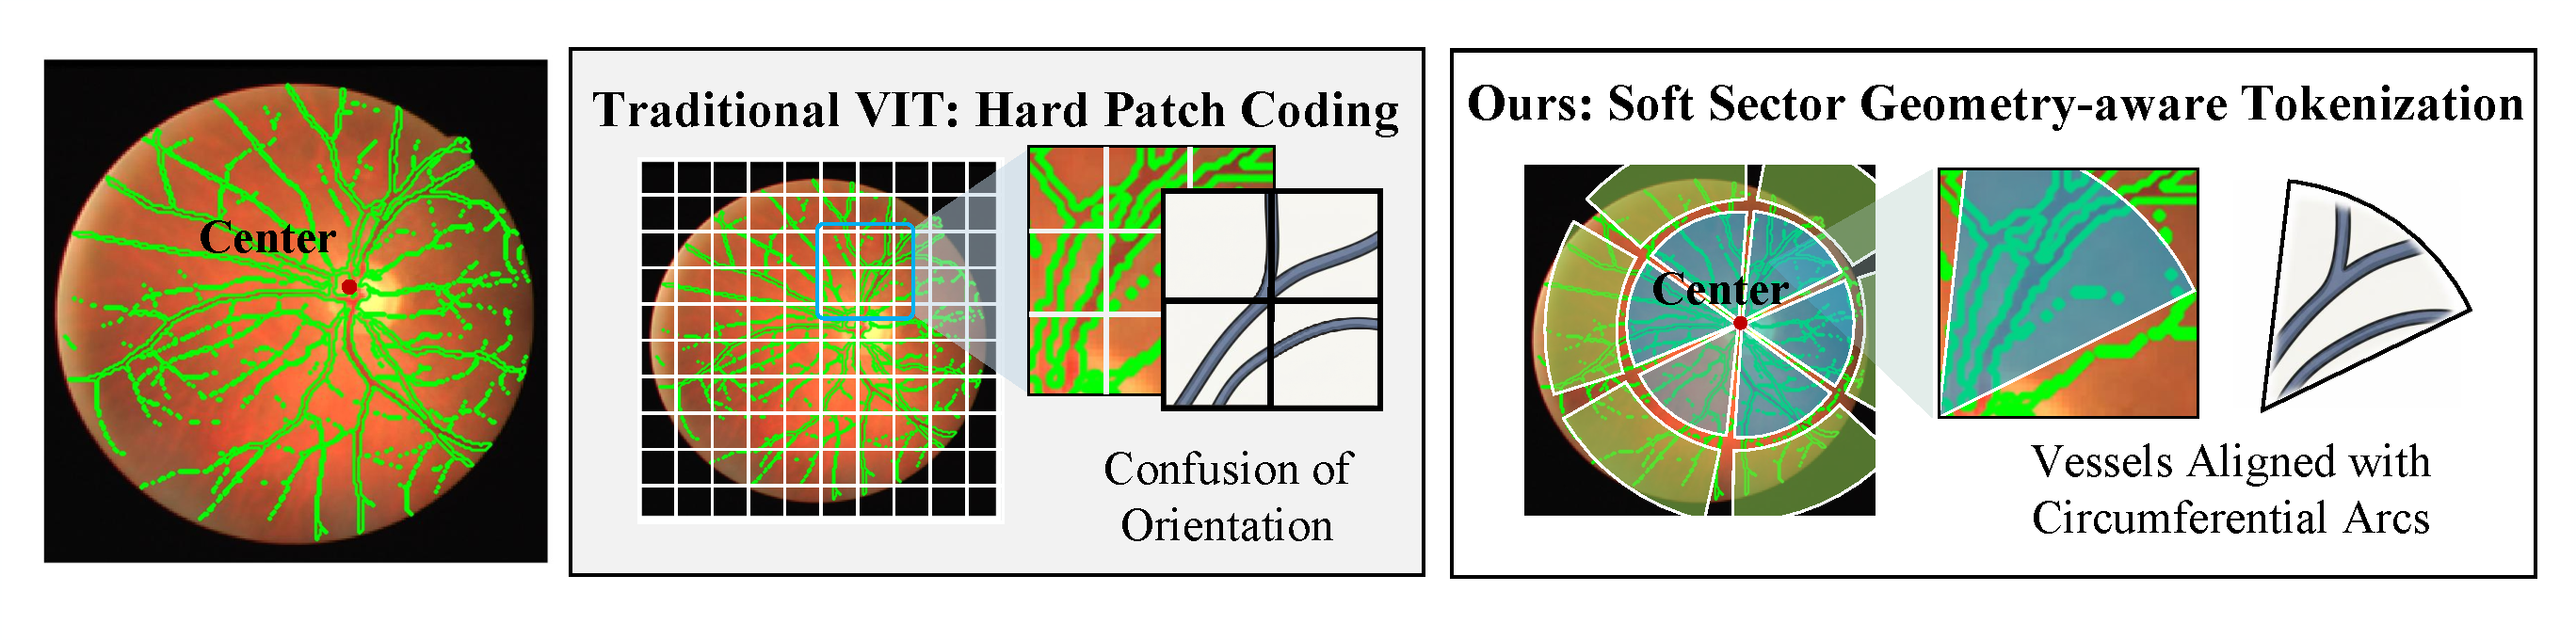
\includegraphics[width=\linewidth]{fig01-sgc-motivation.pdf}
    \caption{Motivation for center-conditioned sector organization. The left panel marks the reference center used to describe retinal vessel geometry. The middle panel illustrates fixed Cartesian patch coding, which does not explicitly represent the relation between vessel orientation and the reference center. The right panel illustrates a soft sector representation that organizes locations by their angular and radial relations to the center.}
    \label{fig:yingyan3}
\end{figure}

Figure~\ref{fig:yingyan3} contrasts fixed Cartesian patches with a center-conditioned representation.
A regular patch grid groups pixels by absolute image location and does not explicitly account for changes in vessel orientation across the retinal field.
The sector representation instead describes each location through its angular and radial relation to a reference center.
Soft membership also allows locations near a sector boundary to contribute without an abrupt reassignment.
This contrast motivates the use of explicit geometric organization for vessels whose local direction changes with spatial position.

Recent retinal vessel segmentation methods have introduced directional representations, topological constraints, and local geometric modeling to better capture vessel anisotropy and connectivity\cite{qiu2024gke,li2025direction,wei2023orientation}.
Polar features provide another means of describing retinal structures relative to a reference location\cite{rezatofighi2009polar}.
Other work redesigns information transfer between the encoder and decoder through gating, channel interaction, or multiscale coordination\cite{wang2022uctransnet,peng2025u}.
Within the methods reviewed here, these directions are typically addressed separately, leaving an explicit structural reference, spatially varying directional organization, and selective transfer of detail at high resolution insufficiently connected.

Three requirements remain insufficiently addressed.
First, feature organization needs an explicit and computable reference.
The retinal vascular tree exhibits a broad radial arrangement around the optic disc region, yet Cartesian representations do not directly express the angular and radial relation between a location and this anatomical context.
Second, the representation must preserve local directional consistency while allowing vessel orientation to change across the retinal field.
A location-independent neighborhood pattern is poorly matched to this combination of local order and global variation.
Third, the decoder must recover fine vessel detail without importing texture noise and pseudo-boundary responses from shallow encoder features.
Unfiltered skip fusion can preserve useful spatial information and irrelevant high-frequency responses at the same time.
A unified model should therefore connect structural anchoring, geometric feature organization, and controlled detail reconstruction.

To meet these requirements, we propose EGCS-Net, the Explicit Geometry-Conditioned Segmentation Network.
EGCS-Net formulates retinal vessel segmentation as geometry-conditioned structure recovery within a dual-branch coarse-to-fine framework.
The structure-prior branch estimates global vessel structure and supplies geometric conditions, while the detail-refinement branch reconstructs the final vessel map through cascaded and same-scale feature injection.
The main contributions are summarized as follows:

\begin{itemize}[label=\textbf{\textbullet}]
    \item We introduce Reference Center Elicitation (RCE), which estimates a learned center state and its reliability from image features. This state provides the computable reference required for subsequent geometric organization.

    \item We develop Sector Geometry Conditioning (SGC), which constructs dual-ring soft sectors around the RCE state and models angular and radial relations among sector representations. SGC organizes locally consistent vessel directions while allowing orientation to vary across the retinal field.

    \item We construct a structure-guided dual-branch framework and integrate Connectivity-Preserving Skip Purification (CSP) at the final high-resolution self-skip. The framework transfers coarse and geometry-enhanced structural cues to the detail-refinement branch, while CSP filters skip information before final reconstruction.
\end{itemize}

The three components form an ordered mechanism.
RCE supplies the reference state required by SGC, SGC produces geometry-enhanced structural features, and CSP controls the final injection of detail at high resolution.
This chain distinguishes EGCS-Net from approaches that add independent feature interaction modules or simply cascade coarse and fine predictions.

The remainder of this paper is organized as follows.
Section 2 reviews related segmentation, geometric modeling, and skip-connection methods.
Section 3 presents the EGCS-Net architecture and its components.
Section 4 describes the experimental protocol and reports the comparative, transfer, ablation, and visualization results.
Section 5 discusses computational cost, limitations, and future directions, and Section 6 concludes the paper.

\section{Related Work}
\label{related_work}

\subsection{General Medical Image Segmentation Frameworks}

U-Net established the symmetric encoder-decoder architecture with cross-level skip connections as a standard foundation for biomedical image segmentation\cite{ronneberger2015u}.
UNet++ introduced nested skip pathways, UNet 3+ aggregated full-scale features, and U-Net v2 reconsidered the design of skip connections\cite{zhou2018unet++,huang2020unet,peng2025u}.
DeepLabv3+ combined atrous convolution with an encoder-decoder design to enlarge contextual coverage while retaining boundary detail\cite{chen2018encoder}.
These approaches established multiscale fusion and spatial-detail transfer as central design concerns.

Transformer-based architectures extend this line of work by modeling interactions over a wider spatial range.
TransUNet, LeViT-UNet, and MT-UNet incorporate Transformer components into U-shaped segmentation frameworks\cite{chen2024transunet,xu2023levit,wang2022mixed}.
FAT-Net, DBUNet, HiFormer, Swin-Unet, and HCT-Unet explore feature-adaptive interaction, dual decoding, hierarchical multiscale representation, pure Transformer processing, and hybrid CNN-Transformer modeling, respectively\cite{wu2022fat,wang2023dual,heidari2023hiformer,cao2022swin,fan2025hct}.
Across these designs, broader context is combined with convolutional locality or multiscale decoding in different ways.

Although these frameworks improve generic feature representation, most organize information on Cartesian feature grids and optimize dense pixel prediction.
For retinal vessels, increased contextual range does not by itself specify a structural reference for feature organization, account for direction changes as a function of image location, or determine which high-resolution skip responses should enter final reconstruction.
The relevance of these requirements becomes clearer in task-specific vessel segmentation methods.

\subsection{Retinal Vessel Segmentation and Ophthalmic Vascular Modeling}

Retinal vessel segmentation methods adapt general backbones to elongated structures, weak contrast, and large variations in vessel width.
SA-Unet adds spatial attention to a lightweight U-Net to refine vessel-relevant responses\cite{guo2021sa}.
OCT$^2$Former uses a dynamic Transformer encoder and a lightweight decoder to capture global vascular context in optical coherence tomography angiography images\cite{tan2023oct2former}.
These methods illustrate two common strategies: selective emphasis of local evidence and wider-range contextual modeling.

Other studies represent vascular structure more directly.
GKE-TUNet embeds skeleton-derived anatomical topology into TransUNet\cite{qiu2024gke}.
DGNet extracts multidirectional features and aggregates globally correlated directional responses for optical coherence tomography angiography vessel segmentation\cite{li2025direction}, whereas OCE-Net combines orientation-aware convolution with local and global context modeling for fundus images\cite{wei2023orientation}.
Earlier work based on polar run-length features transformed local retinal windows into polar coordinates to describe vessels distributed across multiple directions\cite{rezatofighi2009polar}.
Together, these methods show that topology, orientation, and coordinate representation provide task-specific information beyond generic appearance features.

Skip connections form a related line of research because fine-vessel recovery depends on how high-resolution encoder information is transferred to the decoder.
UCTransNet replaces direct U-Net skip transfer with channel-wise multiscale fusion and cross-attention, while U-Net v2 also redesigns skip pathways for medical image segmentation\cite{wang2022uctransnet,peng2025u}.
These designs improve cross-level information transfer, but do not condition skip selection on a learned reference state for retinal vessel geometry.

The reviewed methods separately strengthen local saliency, global context, topology, directionality, coordinate representation, or cross-level fusion.
Among these methods, a learned reference state, center-conditioned angular and radial interaction, and selective high-resolution skip transfer are not integrated as a single dependent process.
EGCS-Net connects these operations in an ordered mechanism: RCE estimates the reference state, SGC organizes features through dual-ring soft sectors, and CSP filters the final high-resolution self-skip before reconstruction.
This organization distinguishes EGCS-Net from methods that address these requirements independently.

\section{Method}
\label{method}

\subsection{Overall Architecture of EGCS-Net}

\subsubsection{Dual-Branch Coarse-to-Fine Architecture}

The overall architecture and information flow of EGCS-Net are shown in Figure~\ref{fig:liuct}.

\begin{figure}[pos=!htbp]
    \centering
    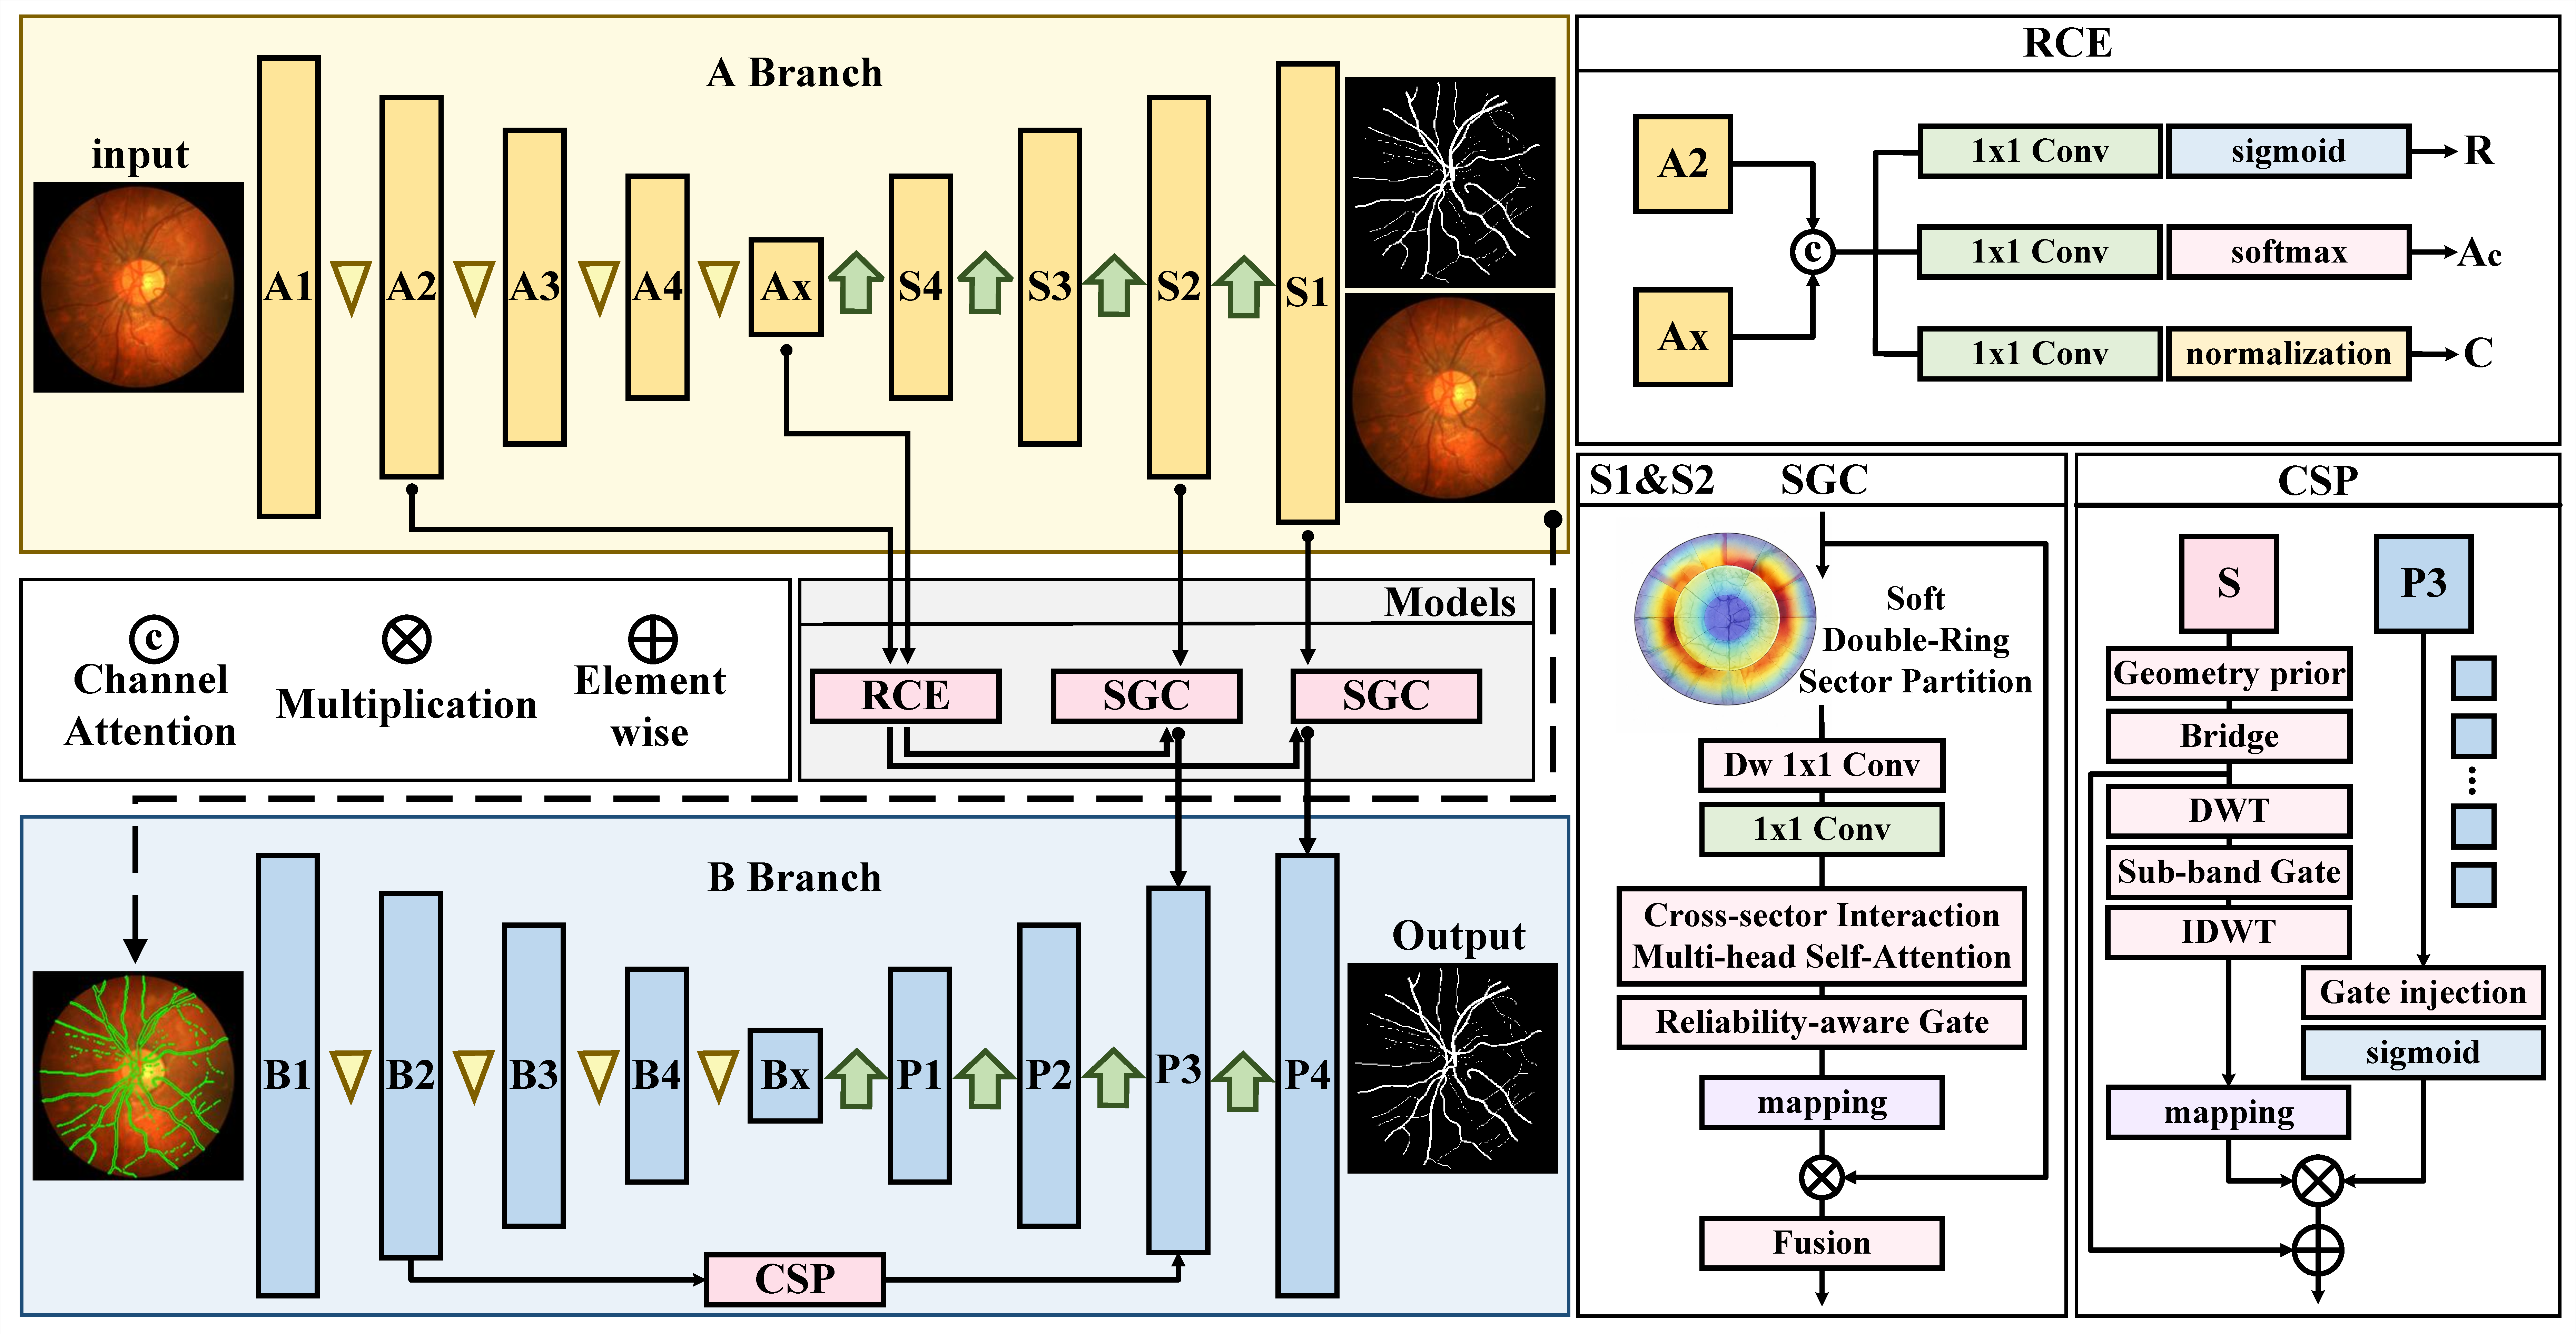
\includegraphics[width=\linewidth]{fig02-egcs-architecture.pdf}
    \caption{Overall architecture and information flow of EGCS-Net. The labels A Branch and B Branch in the diagram correspond to the structure-prior branch and the detail-refinement branch, respectively. The dashed arrow denotes input-level cascaded injection of the coarse prediction, while the solid arrows from SGC to the detail-refinement branch denote same-scale structural injection. RCE uses an intermediate feature and a bottleneck feature to estimate the center response map \(A_c\), radial state \(R\), and reference center \(c\), labeled C in the diagram. SGC constructs dual-ring soft sectors, models cross-sector interactions, and applies reliability-aware feature fusion. CSP uses the shallow skip and decoder features to purify the final high-resolution self-skip before reconstruction. The right panels summarize the internal processing of RCE, SGC, and CSP.}
    \label{fig:liuct}
\end{figure}

Figure~\ref{fig:liuct} presents an ordered flow from structural estimation to detail reconstruction.
Reference Center Elicitation (RCE) supplies the reference state required by Sector Geometry Conditioning (SGC), SGC transfers geometry-enhanced structural features to the detail-refinement branch, and Connectivity-Preserving Skip Purification (CSP) controls the high-resolution skip information used in the final recovery stage.

Given an input color fundus image \(x \in \mathbb{R}^{3 \times H \times W}\), EGCS-Net predicts a vessel probability map through a structure-prior branch and a detail-refinement branch.
The structure-prior branch estimates the whole-image vessel distribution and generates the reference state and geometry-enhanced features used for structural guidance.
The detail-refinement branch receives this guidance through input-level and decoder-level injection and reconstructs the final high-resolution prediction.
The final network prediction is defined as
\begin{equation}
    \hat{y} = \sigma(z_{\mathrm{dr}}), \qquad \hat{y} \in [0,1]^{H \times W}.
    \label{eq:overall-prediction}
\end{equation}
where \(z_{\mathrm{dr}}\) denotes the logit map produced by the detail-refinement branch, and \(\sigma(\cdot)\) is the sigmoid activation function.

The two branches therefore have complementary functions.
The structure-prior branch supplies global structural guidance, whereas the detail-refinement branch combines that guidance with high-resolution features to recover vessel boundaries and fine branches.
This division establishes the coarse-to-fine processing path used by the subsequent modules.

\subsubsection{Structure-Guided Cross-Branch Injection}

EGCS-Net transfers structural information from the structure-prior branch to the detail-refinement branch through two pathways.
Input-level cascaded injection supplies the coarse prediction before feature encoding, while decoder-level same-scale injection supplies geometry-enhanced features during reconstruction.

For input-level cascaded injection, the coarse vessel prediction is projected into the input space and combined with the original image:
\begin{equation}
    x_{\mathrm{dr}} = x + \alpha_{\mathrm{inj}} P(\sigma(z_{\mathrm{sp}})).
    \label{eq:input-cascade}
\end{equation}
where \(z_{\mathrm{sp}}\) denotes the coarse segmentation logit map produced by the structure-prior branch, \(P(\cdot)\) is a \(1 \times 1\) projection convolution, and \(\alpha_{\mathrm{inj}}\) controls the injection strength.
The resulting \(x_{\mathrm{dr}}\) provides the detail-refinement branch with the original image and the projected coarse structural prior.

For decoder-level same-scale injection, SGC enhances two designated decoder features in the structure-prior branch, producing \(a_3\) and \(a_4\).
These features are spatially aligned with the corresponding stages of the detail-refinement branch and are added through residual connections.
The two decoder stages are expressed as
\begin{equation}
    b_3 = \Phi_3([CSP(s_2, p_3), p_3]) + \alpha_{s3} a_3,
    \label{eq:decoder-b3}
\end{equation}
\begin{equation}
    b_4 = \Phi_4([s_1, p_4]) + \alpha_{s4} a_4.
    \label{eq:decoder-b4}
\end{equation}
where \(b_3\) and \(b_4\) are the outputs of the corresponding detail-refinement decoder stages.
The symbols \(s_1\) and \(s_2\) denote encoder skip features, while \(p_3\) and \(p_4\) denote the upsampled decoder features.
The features \(a_3\) and \(a_4\) are generated by the structure-prior branch after SGC enhancement.
The functions \(\Phi_3\) and \(\Phi_4\) denote local fusion modules, \([\cdot,\cdot]\) denotes channel-wise concatenation, and \(\alpha_{s3}\) and \(\alpha_{s4}\) control the two residual injections.

Equation~\eqref{eq:decoder-b3} applies CSP to \(s_2\) under the guidance of \(p_3\) before local fusion and adds the same-scale structural feature \(a_3\).
Equation~\eqref{eq:decoder-b4} fuses \(s_1\) with \(p_4\) and then adds \(a_4\).
Together with the input-level pathway in Equation~\eqref{eq:input-cascade}, these operations supply structural guidance before encoding and at two decoder stages.

\subsubsection{Functional Placement of RCE, SGC, and CSP}

RCE, SGC, and CSP operate at different points in the architecture because they act on different forms of information.
RCE uses intermediate and bottleneck features from the structure-prior branch to estimate the reference state before geometric organization.
SGC is applied at two decoder stages of the same branch, where it models angular and radial relationships with respect to that reference and produces \(a_3\) and \(a_4\).
CSP is placed in the final high-resolution self-skip of the detail-refinement branch, where it filters the skip feature before local fusion and final reconstruction.

These placements define a sequential dependency among the three modules.
RCE provides the reference state used by SGC, SGC generates geometry-enhanced structural features for same-scale cross-branch injection, and CSP controls the local detail entering the final recovery path.
The following subsections describe this sequence beginning with the reference state estimated by RCE.

\subsection{Reference Center Elicitation (RCE)}

Sector-based geometric organization requires each spatial location to be described relative to a shared origin.
Reference Center Elicitation (RCE) constructs an image-specific reference state from features in the structure-prior branch and estimates how strongly that state should influence subsequent geometric processing.
The complete center-state estimation and reliability-control flow is shown in Figure~\ref{fig:modal1}.

\begin{figure}[pos=!htbp]
    \centering
    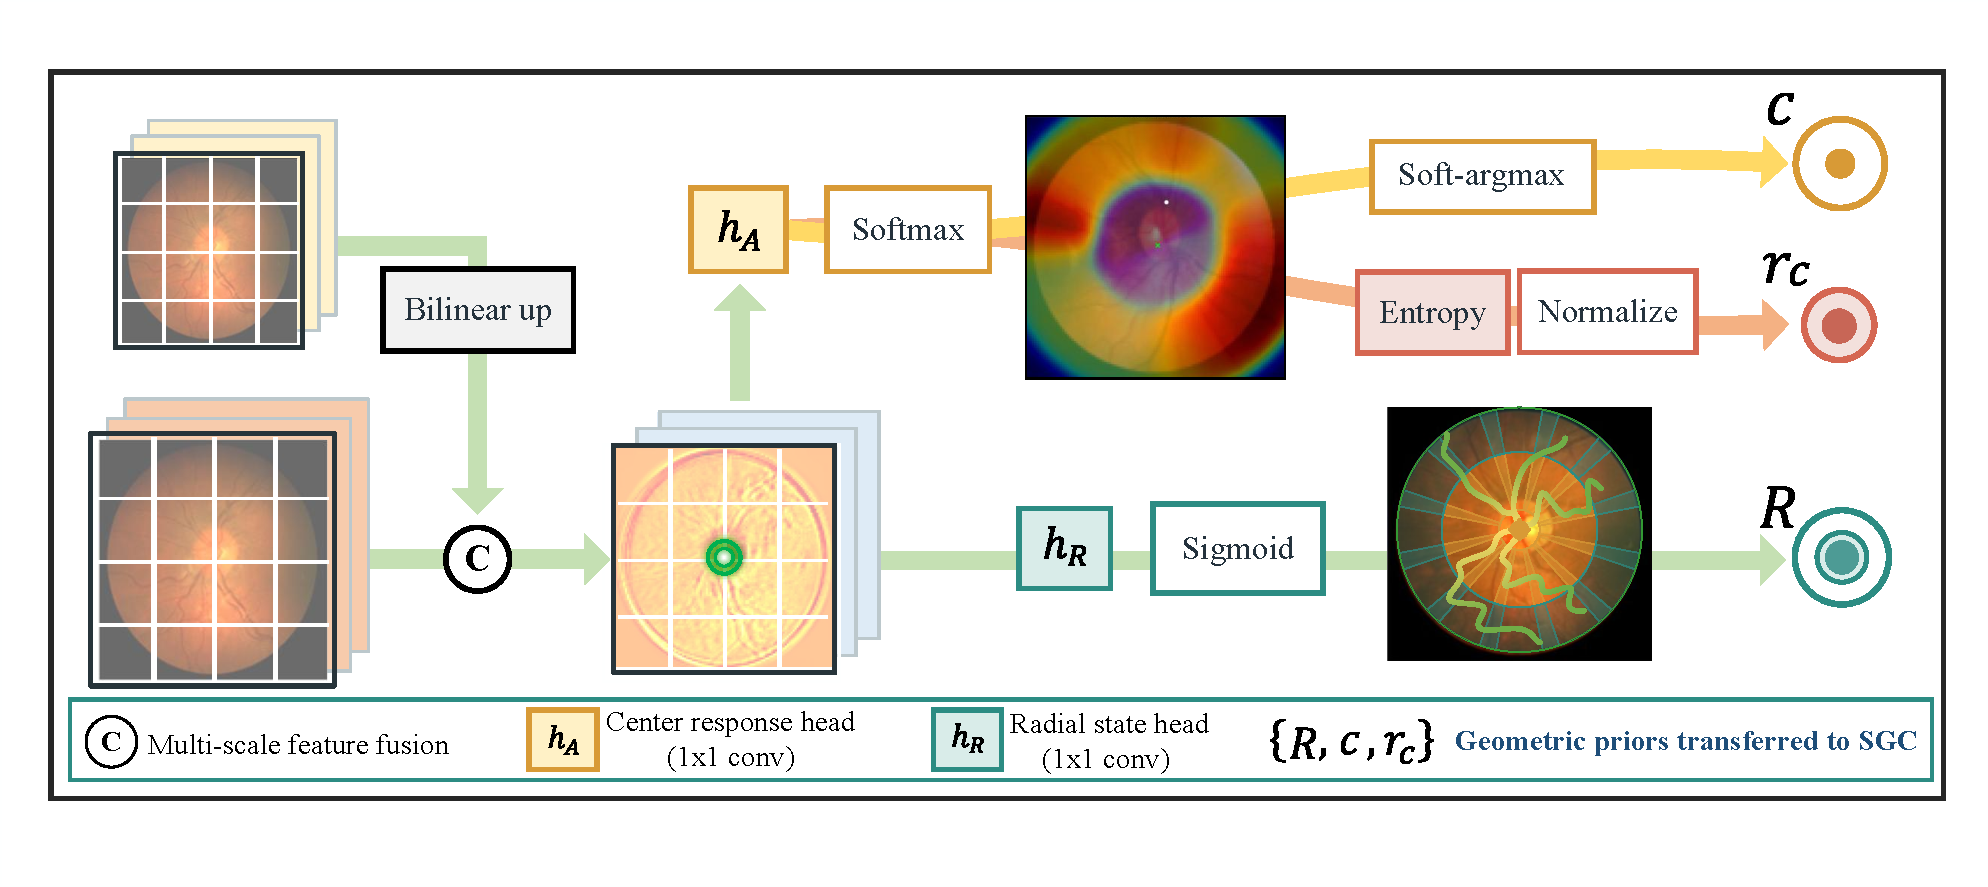
\includegraphics[width=\linewidth]{fig04-rce-module.pdf}
    \caption{Overview of Reference Center Elicitation. From the fused feature \(f_c\), the parallel heads \(h_R\), \(h_A\), and \(g\) estimate radial responses, center logits, and a normalized coordinate representation, respectively. Sigmoid activation produces the radial response map \(R\), spatial softmax produces the center response map \(A_c\), and response-weighted coordinate aggregation yields the reference center \(c\). The concentration of \(A_c\) determines the center reliability \(r_c\), which regulates the subsequent use of the center state. The multiplication symbol denotes response-weighted coordinate aggregation.}
    \label{fig:modal1}
\end{figure}

Figure~\ref{fig:modal1} is read from left to right.
The \(h_R\) path produces \(R\) after sigmoid activation, the \(h_A\) path produces \(A_c\) after spatial softmax, and the \(g\) path supplies the normalized coordinate representation used with \(A_c\) to obtain \(c\).
The reliability path evaluates the concentration of \(A_c\) to obtain \(r_c\).
This separation distinguishes the estimated geometric state from the reliability term that controls its use in subsequent processing.
The resulting state comprises \(A_c\), \(c\), \(R\), and \(r_c\) and provides the condition required by SGC rather than an independently supervised anatomical localization output.

\subsubsection{Reference Center as a Geometric Anchor}

Retinal vessel trajectories exhibit a broad radial arrangement, but their apparent origin can vary with the field of view and image cropping.
Fixed Cartesian coordinates therefore do not provide a consistent basis for describing angular and radial relationships across samples.
RCE addresses this requirement by deriving the reference center \(c\) from the current image features.

The reference center is a continuous coordinate obtained from a learned spatial response distribution.
It is not a ground-truth optic-disc center, and RCE does not perform optic-disc segmentation.
Once \(c\) has been established, SGC can describe feature locations relative to a common origin and organize them by angular direction and radial position.
RCE thus supplies a computable geometric condition for SGC without introducing a separate anatomical localization objective.

\subsubsection{Center State from Multi-Scale Features}

RCE combines an intermediate feature and a bottleneck feature from the structure-prior branch.
Let \(a_2\) denote the intermediate feature and \(a_b\) the bottleneck feature.
The bottleneck feature is upsampled and fused with \(a_2\) as
\begin{equation}
    f_c = \phi_c([a_2, Up(a_b)]).
    \label{eq:rce-feature-fusion}
\end{equation}
where \(f_c\) is the fused center-state feature, \([\cdot,\cdot]\) denotes channel-wise concatenation, \(Up(\cdot)\) denotes bilinear upsampling, and \(\phi_c(\cdot)\) is the center-state estimation subnetwork.

From \(f_c\) in Equation~\eqref{eq:rce-feature-fusion}, RCE derives the center response map, reference center, and radial response map:
\begin{equation}
    A_c = \operatorname{Softmax}(h_A(f_c)),\qquad
    c = \sum_u A_c(u) g(u),\qquad
    R = \sigma(h_R(f_c)).
    \label{eq:rce-center-state}
\end{equation}
where \(u\) indexes a location on the \(H_c \times W_c\) feature lattice.
The head \(h_A(\cdot)\) predicts center logits, and the spatial softmax normalizes these logits to produce the response distribution \(A_c\).
The vector \(g(u)\) denotes the normalized coordinate representation associated with location \(u\), making \(c\) the response-weighted coordinate expectation obtained by soft-argmax.
The head \(h_R(\cdot)\) predicts the radial responses, and \(\sigma(\cdot)\) maps them to the radial response map \(R\).

The spatial interpretation of the three RCE outputs is shown in Figure~\ref{fig:N}.

\begin{figure}[pos=!htbp]
    \centering
    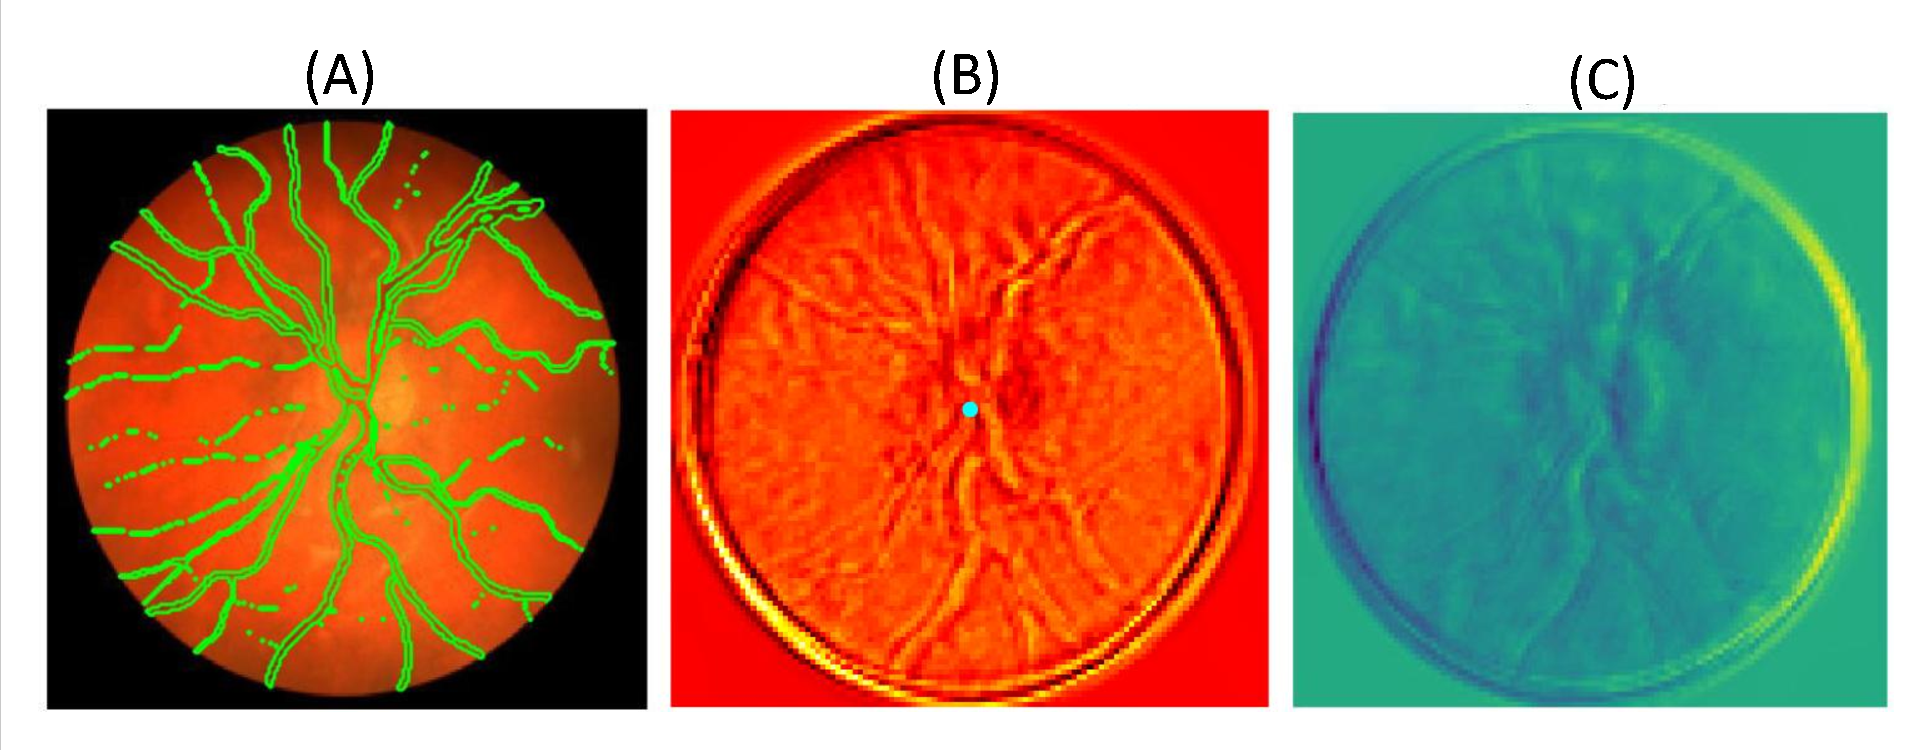
\includegraphics[width=0.90\linewidth]{fig03-rce-center-visualization.pdf}
    \caption{Visualization of the RCE center state. \textbf{(A)} The fundus sample used for visualization. \textbf{(B)} The center response map \(A_c\), with the marker indicating the reference center \(c\) obtained by soft-argmax. \textbf{(C)} The radial response map \(R\) used in subsequent geometry-conditioned aggregation.}
    \label{fig:N}
\end{figure}

Panel (A) identifies the sample associated with the visualization.
Panel (B) shows how \(A_c\) distributes center responses over the image and how their weighted expectation determines \(c\).
Panel (C) shows the radial response map \(R\), which provides spatial weighting for subsequent sector aggregation.
Together, \(A_c\) and \(c\) establish the geometric origin, while \(R\) supplies the radial weighting used by SGC.

\subsubsection{Reliability-Controlled Center Usage}

The reliability path in Figure~\ref{fig:modal1} addresses uncertainty in the learned spatial reference.
Because subsequent sector relationships are organized relative to \(c\), a diffuse center response can provide a less determinate reference.
RCE measures the concentration of \(A_c\) using normalized spatial entropy:
\begin{equation}
    r_c = 1 - \frac{H(A_c)}{\log(H_c W_c)}.
    \label{eq:rce-reliability}
\end{equation}
where \(H(A_c)\) is the Shannon entropy of the spatial distribution \(A_c\), \(H_c\) and \(W_c\) are its spatial dimensions, and \(\log(H_c W_c)\) is the maximum entropy for a distribution over that lattice.
Equation~\eqref{eq:rce-reliability} therefore maps a concentrated response to a larger \(r_c\) and a dispersed response to a smaller \(r_c\).

The reliability \(r_c\) does not re-estimate \(c\).
In the subsequent reliability-guided feature projection of SGC, \(r_c\) provides a sample-level gating factor, while token-level confidence controls local feature write-back.
The two factors regulate how strongly geometry-enhanced information is returned to the feature map when the estimated reference is uncertain.
The resulting reliability-aware center state provides the reference condition used by SGC in the next stage.

\subsection{Sector Geometry Conditioning (SGC)}

Sector Geometry Conditioning (SGC) converts the reference state estimated by RCE into an explicit organization of angular and radial relationships.
Given an input feature map \(X\), the reference center \(c\), and the radial response map \(R\), SGC assigns spatial features to dual-ring soft sectors, aggregates sector-specific tokens, models interactions among these tokens, and returns the resulting structural information to the feature map under reliability control.
The core geometric processing stages are shown in Figure~\ref{fig:modal2}.

\begin{figure}[pos=!htbp]
    \centering
    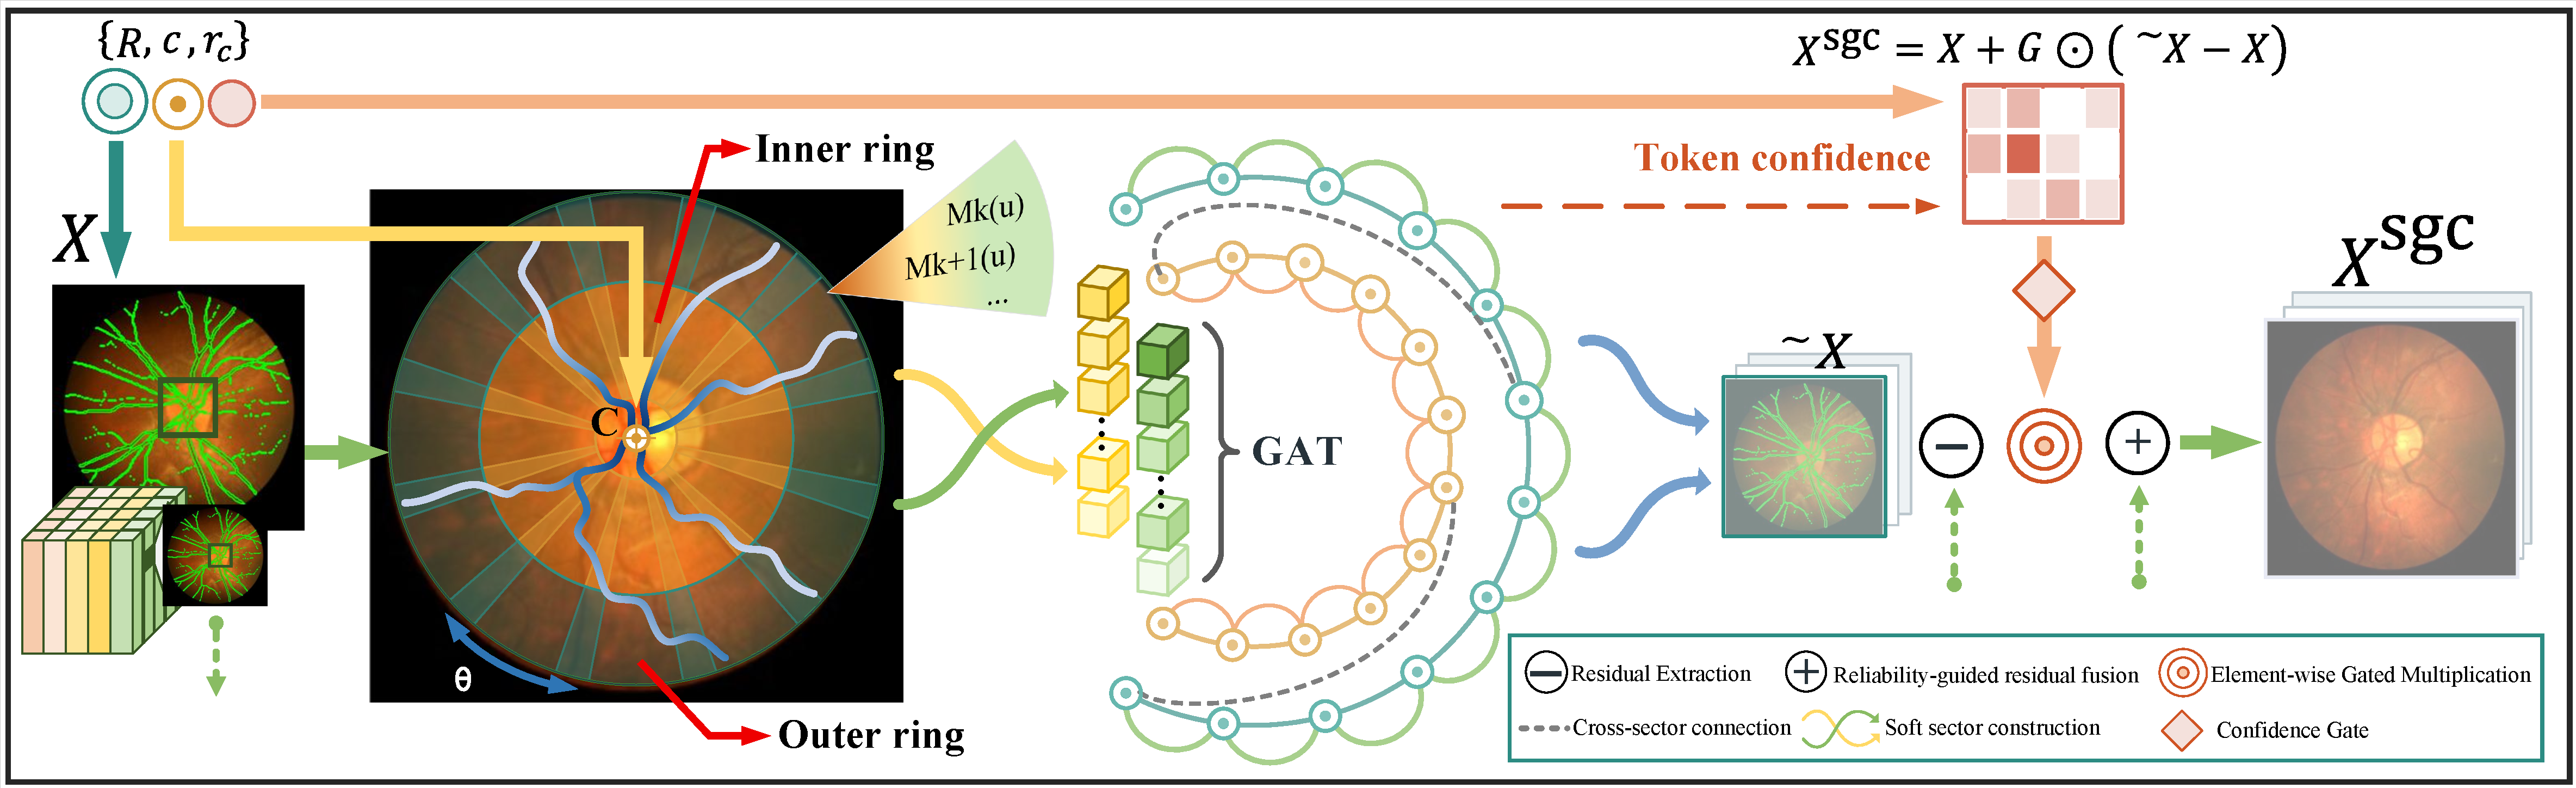
\includegraphics[width=\linewidth]{fig05-sgc-module.pdf}
    \caption{Core geometric processing stages of SGC. Soft Sector Construction (SSC) organizes features into inner-ring and outer-ring sectors around the reference center \(c\). Geometry-Aware Tokenization (GAT) aggregates sector-specific tokens, and Cross-Sector Interaction (CSI) models angular continuity, radial transmission, and cross-sector consistency.}
    \label{fig:modal2}
\end{figure}

Figure~\ref{fig:modal2} summarizes the geometric processing path from SSC to GAT and CSI.
SSC first assigns the spatial features to sectors defined by their angular direction and radial range.
GAT then converts these spatially distributed features into sector tokens, after which CSI exchanges information among tokens with related geometric identities.
The updated token representation is subsequently returned to the spatial feature map through the reliability-guided projection described below.

\subsubsection{Soft Sector Construction}

Soft Sector Construction (SSC) establishes the geometric coordinate system used by SGC.
Taking the reference center \(c\) as the origin, SSC divides the feature domain into an inner ring and an outer ring and partitions each ring into angular sectors.
The ring membership describes the radial range of a location, while the sector membership describes its angular direction relative to \(c\).
Together, these two identities reorganize the Cartesian feature grid into a center-conditioned geometric representation.

SSC uses soft assignment instead of assigning each location exclusively to a single sector.
A location near a sector boundary can therefore contribute to neighboring sectors with different weights.
This treatment avoids an abrupt separation of vessel responses that cross predefined angular boundaries and retains the geometric association between adjacent sectors.
The resulting inner-ring and outer-ring masks are visualized in Figure~\ref{fig:huan}.

\begin{figure}[pos=!htbp]
    \centering
    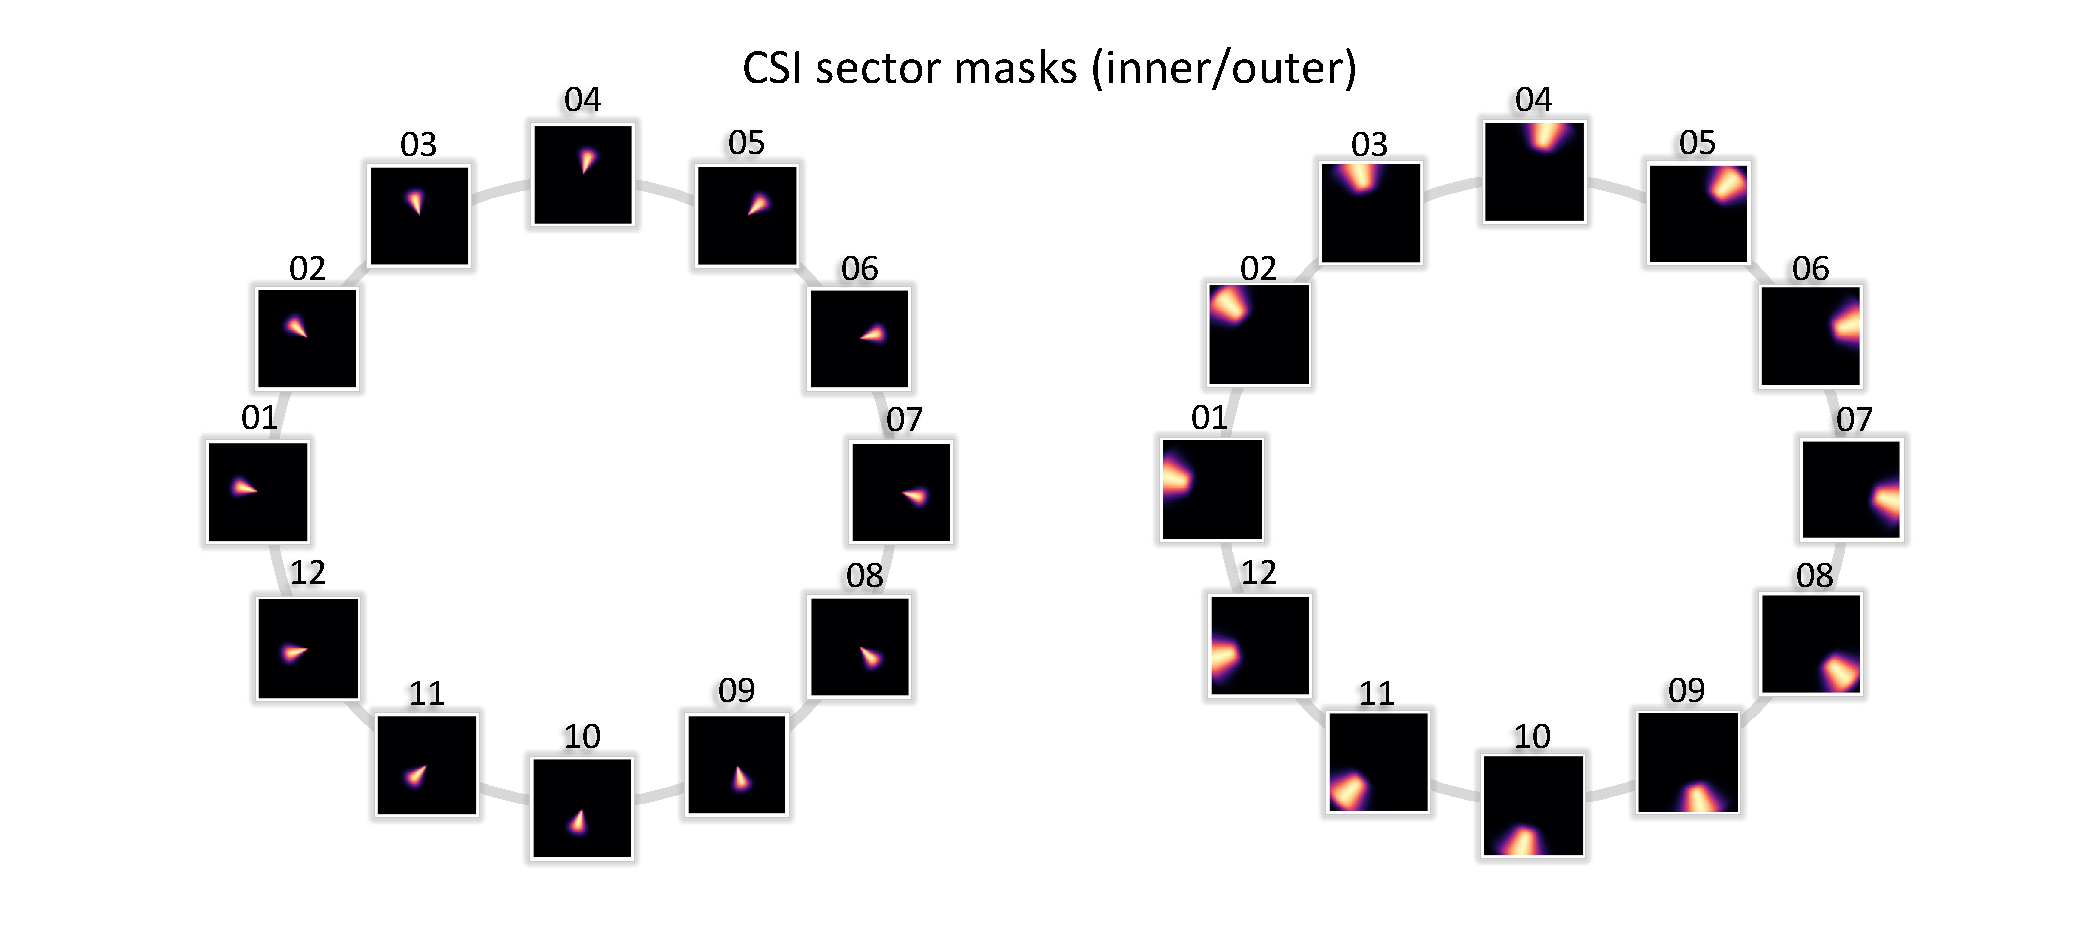
\includegraphics[width=0.86\linewidth]{fig06-sgc-sector-masks.pdf}
    \caption{Visualization of the dual-ring soft sector masks used by SSC. The left and right groups display the 12 inner-ring and 12 outer-ring masks, respectively. Indices 01 through 12 identify corresponding angular sectors in the two radial ranges, and the heat-map intensity represents the soft assignment weight \(M_k(u)\).}
    \label{fig:huan}
\end{figure}

In Figure~\ref{fig:huan}, masks with the same index correspond to the same angular direction but cover different radial ranges.
The inner-ring masks concentrate their support near the reference center, whereas the corresponding outer-ring masks extend the support into the more distant annular region.
The gradual intensity changes at the sector boundaries represent soft membership rather than predicted vessel responses.
Each spatial location can consequently retain weighted associations with neighboring angular sectors while remaining distinguishable by its radial range.

\subsubsection{Geometry-Aware Tokenization}

After the dual-ring masks have been constructed, Geometry-Aware Tokenization (GAT) aggregates the features associated with each sector.
Let \(k\) denote a sector index that incorporates its ring and angular identities.
The token associated with sector \(k\) is calculated by weighted pooling:
\begin{equation}
    t_k = \frac{\sum_u M_k(u) R(u) X(u)}
    {\sum_u M_k(u) R(u) + \varepsilon}.
    \label{eq:sgc-tokenization}
\end{equation}
where \(u\) indexes a spatial location, \(M_k(u)\) is the soft assignment weight of location \(u\) to sector \(k\), \(R(u)\) is the radial response supplied by RCE, \(X(u)\) is the input feature at \(u\), and \(\varepsilon\) is a small positive constant used for numerical stability.

Equation~\eqref{eq:sgc-tokenization} combines the sector membership and radial response when aggregating each token.
The normalization in the denominator accounts for differences in the total assignment weight among sectors.
Because each token remains associated with a particular ring and angular direction, the spatial cues distributed across the original feature grid are represented as geometrically indexed units for subsequent interaction.

\subsubsection{Cross-Sector Interaction (CSI)}

Cross-Sector Interaction (CSI) operates on the sector tokens generated by GAT.
A lightweight multi-head attention block models three complementary relationships among these tokens.
Interactions between neighboring sectors within the same ring describe angular continuity.
Interactions between the inner-ring and outer-ring sectors associated with the same direction describe radial transmission.
Broader interactions among sectors provide contextual information when a vessel trajectory changes direction across the feature domain.

The interaction units in CSI are sector tokens rather than individual grid locations.
Each token therefore carries an angular identity, a radial identity, and a spatial relationship to the reference center.
CSI uses these identities to organize information exchange among structurally related regions while retaining the ability to model dependencies across different directions.
This organization provides the geometry-conditioned token representation used in the following feature-projection stage.

\subsubsection{Reliability-Guided Feature Projection}

The sector tokens updated by CSI are reconstructed as the spatial feature map \(\tilde{X}\).
Instead of directly replacing the original feature map, SGC applies a reliability-controlled residual update:
\begin{equation}
    X^{\mathrm{sgc}} = X + G \odot (\tilde{X} - X).
    \label{eq:sgc-projection}
\end{equation}
where \(X\) is the original feature map, \(\tilde{X}\) is the feature map reconstructed from the updated sector tokens, \(G\) is the write-back gating tensor, and \(\odot\) denotes element-wise multiplication.

The gate \(G\) combines the sample-level center reliability \(r_c\) with token-level confidence information.
When the center response is dispersed and \(r_c\) is small, the contribution of the geometry-conditioned correction is reduced at the sample level.
Token-level confidence further controls the correction at individual spatial locations.
Equation~\eqref{eq:sgc-projection} therefore writes the gated residual \(\tilde{X}-X\) back to the original representation instead of propagating the reconstructed feature map without constraint.

\subsubsection{Placement and Cross-Branch Injection}

SGC is applied at two designated decoder stages of the structure-prior branch.
At each stage, it uses the reference state supplied by RCE to reorganize the current feature map and produce a geometry-conditioned representation.
The resulting features are denoted by \(a_3\) and \(a_4\) in the overall architecture.

As specified in Equation~\eqref{eq:decoder-b3} and Equation~\eqref{eq:decoder-b4}, \(a_3\) and \(a_4\) are transferred to the corresponding stages of the detail-refinement branch through same-scale residual injection.
This transfer supplies the refinement branch with features that have undergone center-conditioned sector construction, geometry-aware tokenization, cross-sector interaction, and reliability-guided projection.
The experimental comparison of alternative SGC placement configurations is reported in the ablation section rather than used to justify the placement within the method definition.

Within the complete EGCS-Net processing chain, RCE establishes the reference state, SGC converts this state into geometry-conditioned structural features, and CSP controls the high-resolution skip information used during final detail reconstruction.

\subsection{Connectivity-Preserving Skip Purification (CSP)}

The final high-resolution skip connection carries spatial detail required for fine-vessel reconstruction, but it can also transfer responses produced by background texture, illumination transitions, and other task-irrelevant high-frequency structures.
Connectivity-Preserving Skip Purification (CSP) filters this information before it enters the final reconstruction stage of the detail-refinement branch.
Given the shallow skip feature \(S\) and the current decoder state, CSP constructs direction-supported bridge candidates through Structure-Consistent Candidate Bridging (SCB), regulates their frequency components through Wavelet-Assisted Purification (WAP), and returns the purified representation through Gated Safe Reinjection (GSR).
The WAP and GSR processing flow, together with the inputs supplied by SCB and the decoder, is shown in Figure~\ref{fig:modal3}.

\begin{figure}[pos=!htbp]
    \centering
    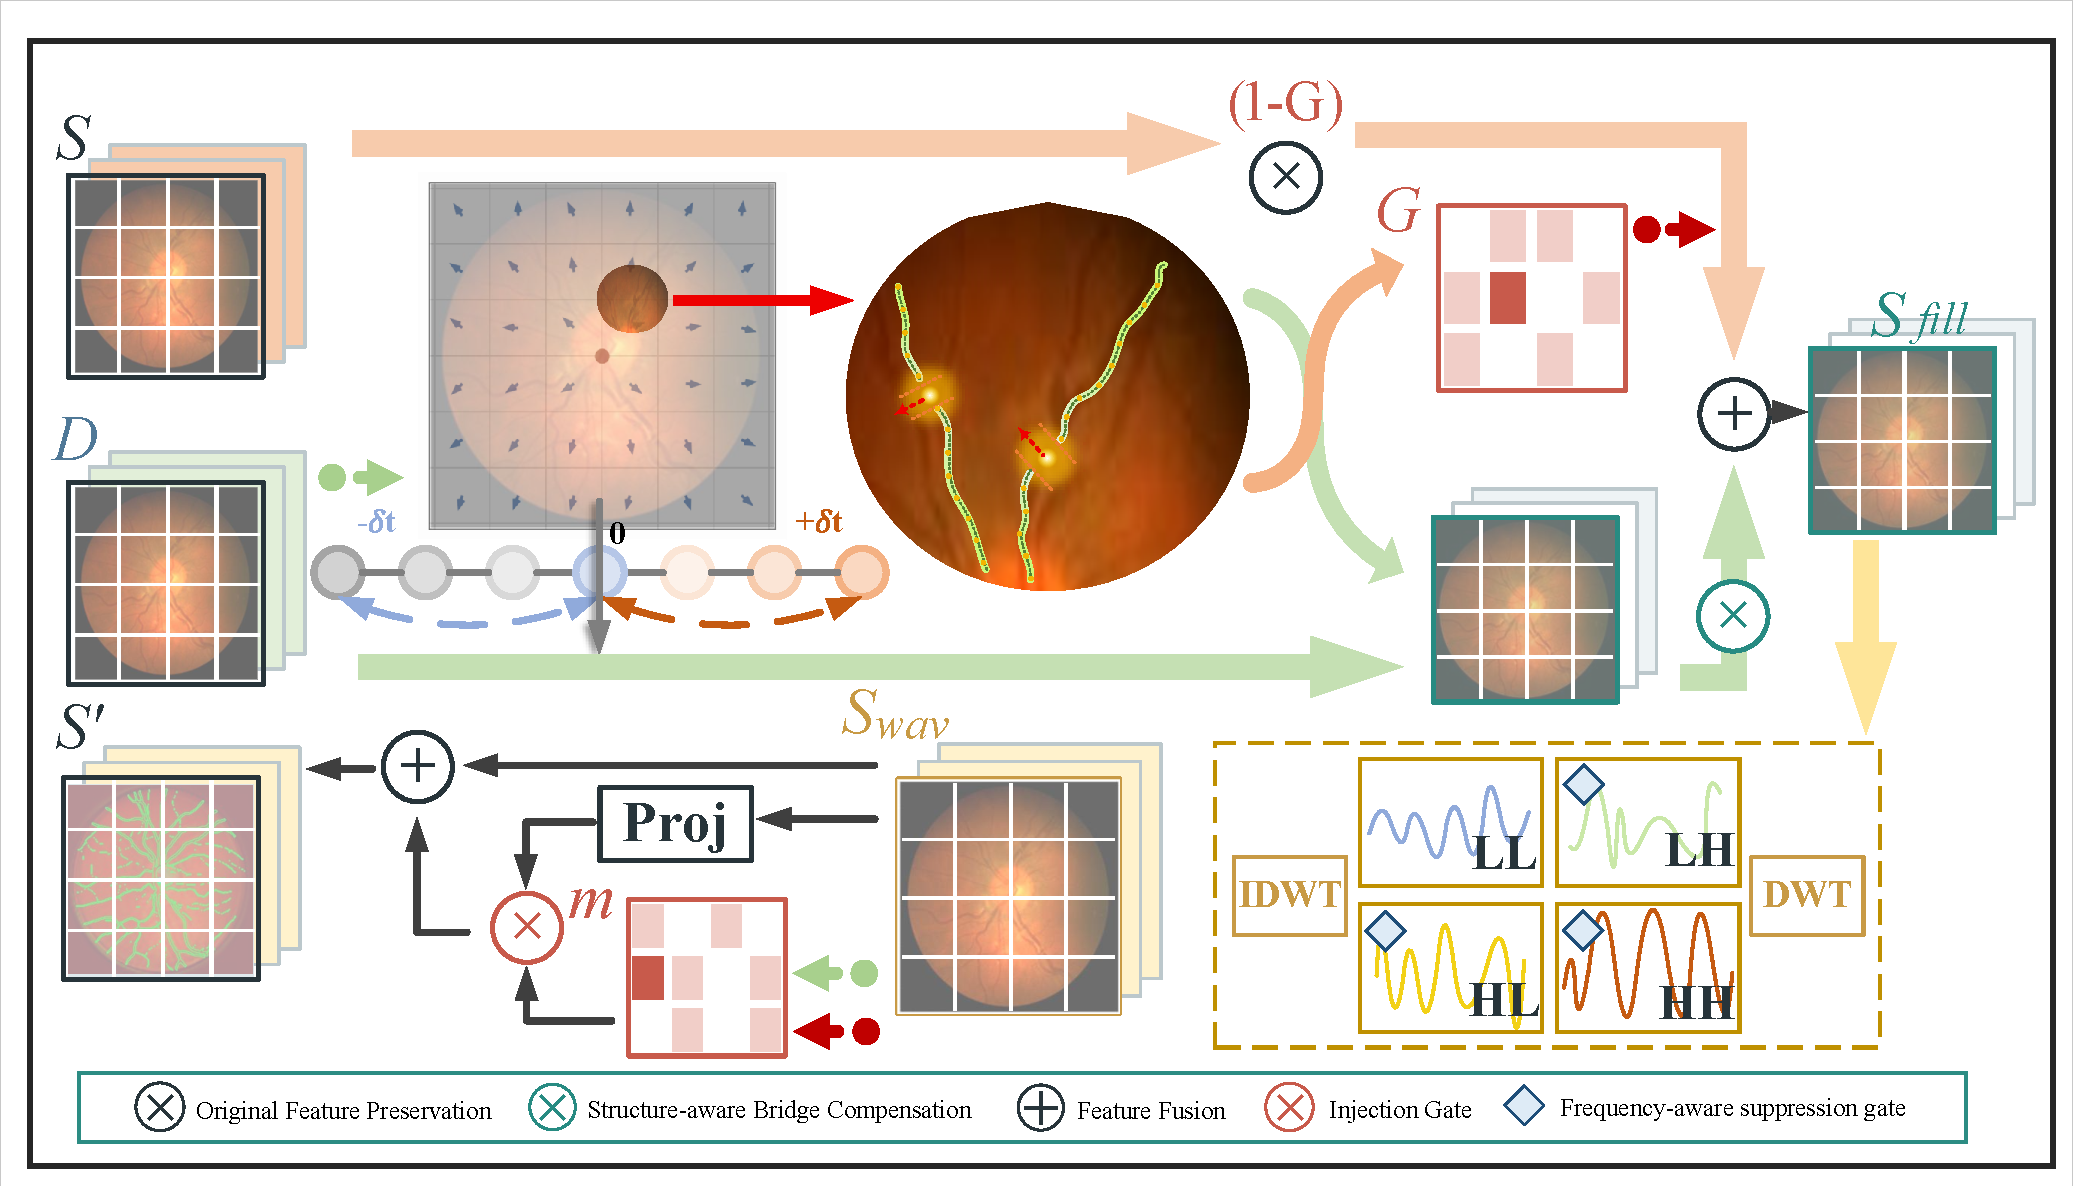
\includegraphics[width=\linewidth]{fig07-csp-module.pdf}
    \caption{Processing and reinjection flow of CSP at the final high-resolution self-skip. SCB produces the compensated skip feature \(S_{\mathrm{fill}}\) and a bridge-confidence representation. WAP applies the Haar discrete wavelet transform (DWT) to \(S_{\mathrm{fill}}\), retains the low-frequency subband \(LL\), modulates the high-frequency subbands \(LH\), \(HL\), and \(HH\), and reconstructs \(S_{\mathrm{wav}}\) through the inverse transform (IDWT). GSR uses \(S_{\mathrm{wav}}\), the current decoder state, and the SCB bridge confidence to generate the injection gate and produce the purified output \(S'\). The multiplication and addition symbols denote element-wise gating and residual addition, respectively.}
    \label{fig:modal3}
\end{figure}

Figure~\ref{fig:modal3} is read from the upper WAP path to the lower GSR path.
WAP receives the compensated skip feature \(S_{\mathrm{fill}}\) from SCB and reconstructs \(S_{\mathrm{wav}}\) after subband-specific modulation.
GSR then combines \(S_{\mathrm{wav}}\) with the current decoder state and bridge confidence.
This sequence separates candidate construction, frequency-domain purification, and controlled reinjection before the skip information is used by the decoder.

\subsubsection{SCB: Structure-Consistent Candidate Bridging}

Structure-Consistent Candidate Bridging (SCB) constructs candidate responses for spatial locations that have weak local activation but are supported by neighboring evidence along an estimated vessel direction.
Given the skip feature \(S\), SCB predicts a local direction vector and derives its tangential and normal components:
\begin{equation}
    v = f_v(S), \qquad
    t = \frac{v}{\lVert v \rVert_2 + \varepsilon}, \qquad
    n = (-t_y, t_x).
    \label{eq:csp-direction-field}
\end{equation}
where \(f_v(\cdot)\) is the direction-prediction function, \(v\) is the predicted direction vector, \(t\) is its normalized tangential direction, \(n\) is the corresponding normal direction, and \(\varepsilon\) is a small positive constant used for numerical stability.

For each offset \(\delta \in \Delta\), SCB samples the skip feature in the positive and negative tangential directions and forms a bridge candidate:
\begin{equation}
    B_\delta = \frac{1}{2}\bigl[GS(S, +\delta t) + GS(S, -\delta t)\bigr].
    \label{eq:csp-bridge-candidate}
\end{equation}
where \(\Delta\) is the set of sampling offsets, \(GS(\cdot)\) denotes bilinear grid sampling, and \(B_\delta\) is the candidate obtained at offset \(\delta\).
Equation~\eqref{eq:csp-bridge-candidate} averages the two tangential samples so that a locally weak position can receive candidate support from both directions along the estimated trajectory.

SCB does not accept every bridge candidate.
Candidate selection considers compatibility with the current decoder state, local directional confidence, and the relation between tangential and normal evidence.
The candidates that satisfy these conditions are aggregated into the bridge representation \(B\), while the bridge gate \(G\) controls their contribution to the original skip feature:
\begin{equation}
    S_{\mathrm{fill}} = (1 - G) \odot S + G \odot B.
    \label{eq:csp-bridge-fusion}
\end{equation}
where \(S_{\mathrm{fill}}\) is the compensated skip representation and \(\odot\) denotes element-wise multiplication.
Equation~\eqref{eq:csp-bridge-fusion} retains the original feature where the bridge gate is small and introduces the candidate representation where directional and decoder evidence support the update.

\subsubsection{WAP: Wavelet-Assisted Purification}

Wavelet-Assisted Purification (WAP) separates low-frequency structural content from high-frequency responses before the skip representation is returned to the decoder.
A Haar wavelet transform decomposes \(S_{\mathrm{fill}}\) into one low-frequency subband and three directional high-frequency subbands.
The high-frequency components are then modulated under constraints supplied by the current decoder state:
\begin{equation}
    S_{\mathrm{wav}} = IDWT(LL,\, g_{LH} \odot LH,\, g_{HL} \odot HL,\, g_{HH} \odot HH).
    \label{eq:csp-wavelet-purification}
\end{equation}
where \(LL\) is the low-frequency subband, \(LH\), \(HL\), and \(HH\) are the three high-frequency subbands, and \(g_{LH}\), \(g_{HL}\), and \(g_{HH}\) are the corresponding band-wise gates.
The inverse discrete wavelet transform \(IDWT(\cdot)\) reconstructs the purified spatial representation \(S_{\mathrm{wav}}\).

The subbands before and after WAP modulation are visualized in Figure~\ref{fig:k}.

\begin{figure}[pos=!htbp]
    \centering
    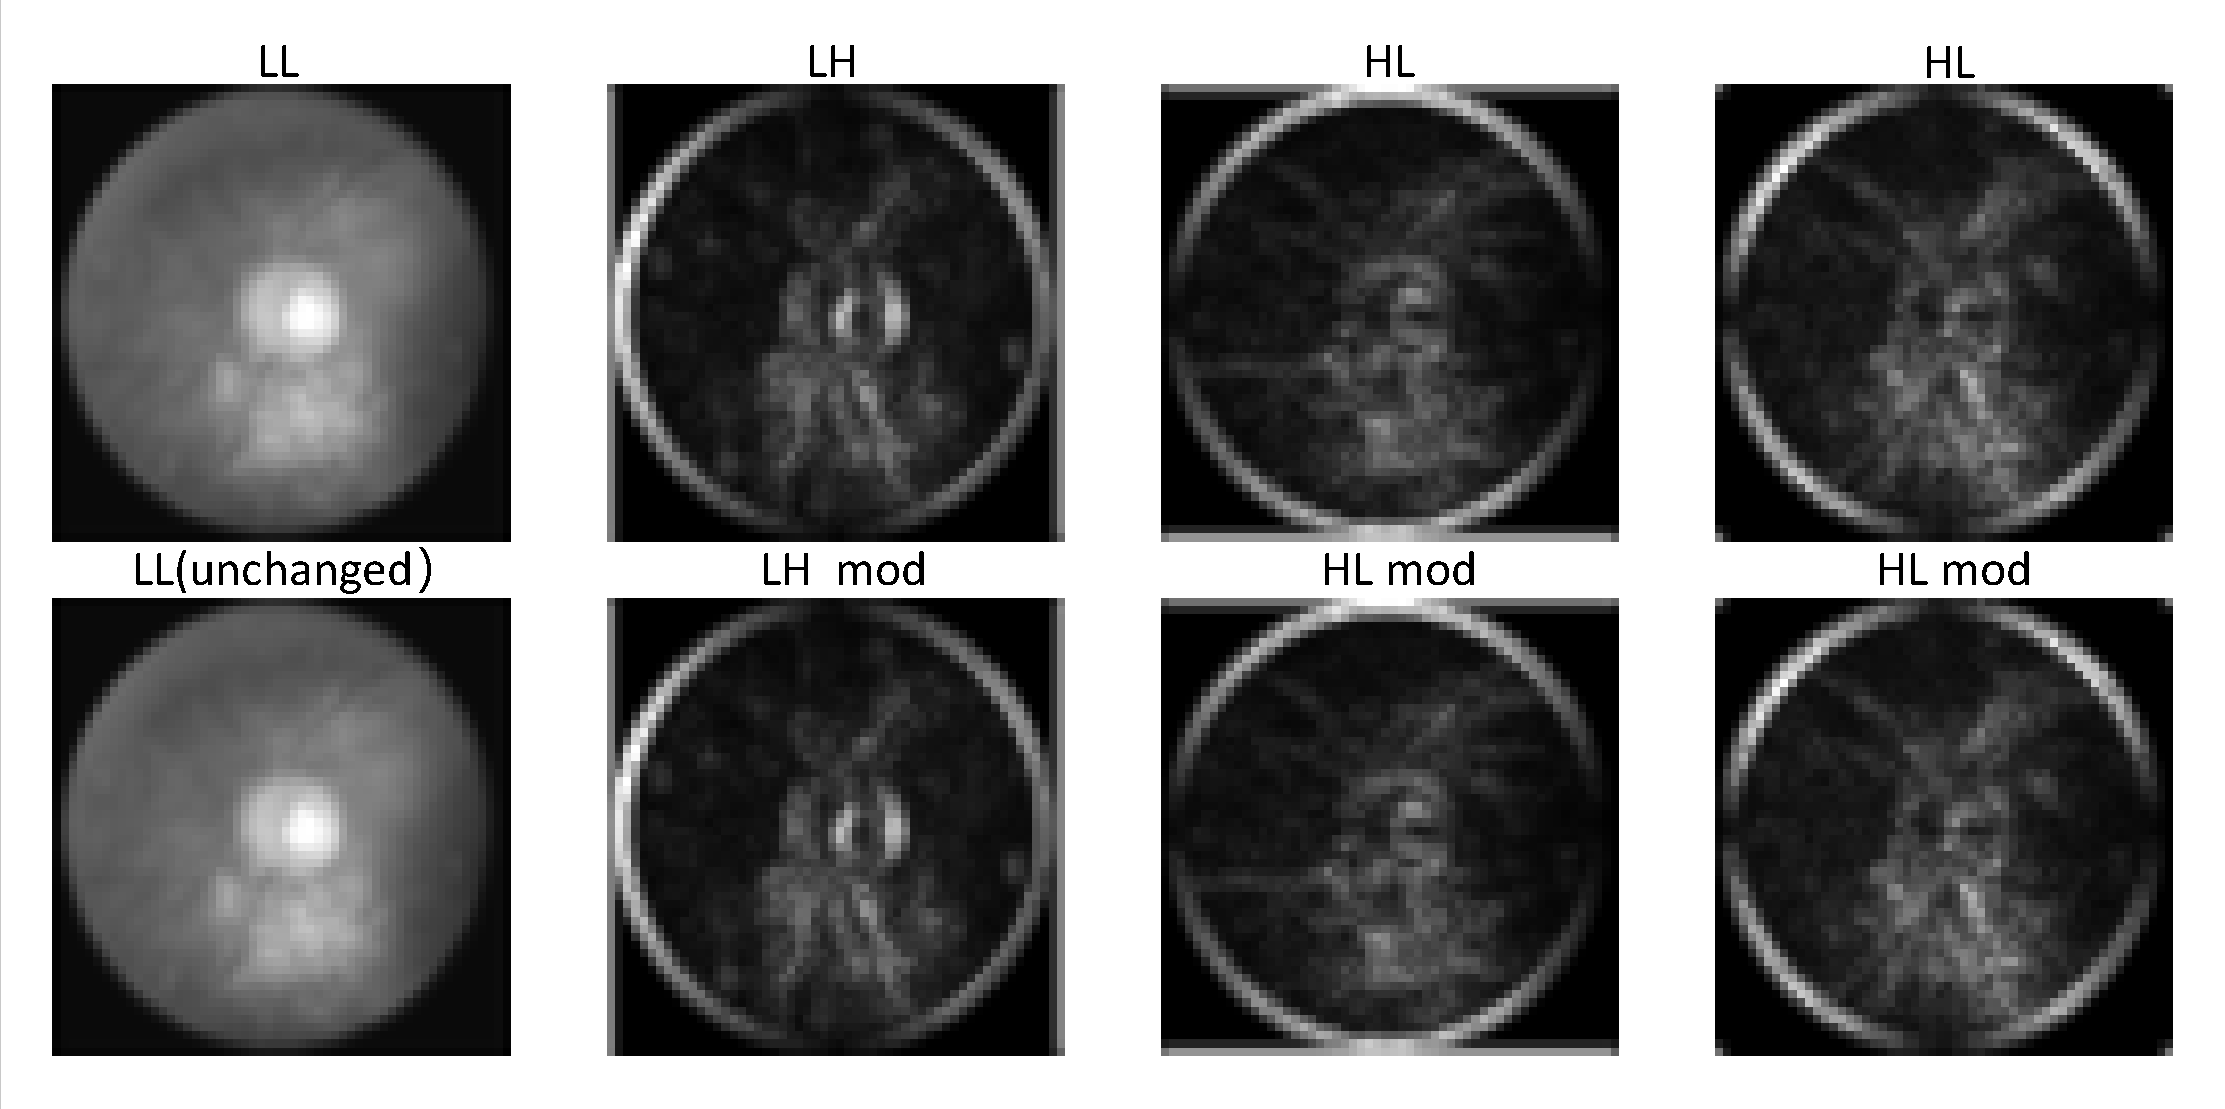
\includegraphics[width=0.85\linewidth]{fig10-sgc-response-map.pdf}
    \caption{Visualization of wavelet subbands before and after WAP modulation. The top row shows the \(LL\), \(LH\), \(HL\), and \(HH\) subbands obtained from the Haar wavelet decomposition of \(S_{\mathrm{fill}}\). The bottom row shows the unchanged \(LL\) subband and the modulated high-frequency components \(g_{LH}\odot LH\), \(g_{HL}\odot HL\), and \(g_{HH}\odot HH\) used to reconstruct \(S_{\mathrm{wav}}\).}
    \label{fig:k}
\end{figure}

Figure~\ref{fig:k} distinguishes the information retained without modification from the frequency components controlled by WAP.
The low-frequency subband preserves the coarse spatial content, whereas the three gated high-frequency subbands regulate directional detail before inverse reconstruction.
This visualization represents the internal frequency decomposition and modulation performed by WAP rather than an SGC response map or a quantitative experiment.

\subsubsection{GSR: Gated Safe Reinjection}

Gated Safe Reinjection (GSR) returns the wavelet-purified representation to the decoder through a controlled residual update.
The injection gate is generated from the current decoder state and the bridge confidence supplied by SCB:
\begin{equation}
    S' = S_{\mathrm{wav}} + m \odot Proj(S_{\mathrm{wav}}).
    \label{eq:csp-safe-reinjection}
\end{equation}
where \(Proj(\cdot)\) denotes channel projection, \(m\) is the injection gate, and \(S'\) is the output of CSP.
Equation~\eqref{eq:csp-safe-reinjection} retains \(S_{\mathrm{wav}}\) as the residual base and controls the projected correction through \(m\).
The decoder state supplies semantic compatibility information, while the bridge confidence indicates whether the local correction is supported by the directional analysis performed in SCB.

\subsubsection{CSP Deployment at the Final High-Resolution Self-Skip}

CSP is applied only to the final high-resolution self-skip of the detail-refinement branch.
As specified in Equation~\eqref{eq:decoder-b3}, CSP processes the encoder feature \(s_2\) under the guidance of the upsampled decoder feature \(p_3\) before the purified skip representation is concatenated with \(p_3\) for local fusion.

This location retains the spatial detail needed for final reconstruction and is also close to the prediction stage, where transferred background responses would have limited opportunity for correction.
Restricting CSP to this entry confines its function to filtering the high-resolution skip information immediately before final recovery.
This entry is denoted S3 in the placement ablation, while comparisons with alternative placements are reported in the experimental section.

CSP completes the ordered processing chain of EGCS-Net.
RCE establishes the structural reference, SGC produces geometry-conditioned features for cross-branch guidance, and CSP controls the local high-resolution information used during final reconstruction.

\section{Experiments}

This section describes the experimental protocol and presents the quantitative comparisons, qualitative results, cross-architecture transfer experiments, and ablation studies used to evaluate EGCS-Net.

\subsection{Experimental Setup}
\label{sec:experimental-setup}

EGCS-Net was evaluated on five publicly available retinal vessel segmentation datasets: DRIVE, STARE, CHASEDB1, AV-WIDE, and ARIA. DRIVE and STARE are established color fundus benchmarks for retinal vessel segmentation \cite{staal2004ridge,hoover2000locating}. CHASEDB1 contains complex branching patterns and fine vessels that provide a demanding setting for structural recovery \cite{fraz2012ensemble}. AV-WIDE extends the evaluation to images with a wider field of view \cite{khanal2020dynamic}. ARIA contains images from healthy subjects and patients with diabetes or age-related macular degeneration, introducing additional variation associated with pathological appearance \cite{farnell2008enhancement}. Together, the five datasets cover differences in vessel caliber, image contrast, field of view, background appearance, and data distribution.

All comparison methods were trained and evaluated separately on each dataset using the same dataset-specific protocol. Within a dataset, the data partition, preprocessing procedure, optimization settings, and testing procedure were kept identical across methods. This controlled setting limits differences in the reported results to changes in the evaluated segmentation model.

Performance was assessed using intersection over union (IoU), Dice score, sensitivity (Sen), specificity (Spe), precision (Pre), area under the receiver operating characteristic curve (AUC), and accuracy (Acc). Dice and IoU were treated as the primary metrics because they measure vessel-region overlap under the foreground-background imbalance of retinal vessel segmentation. Sensitivity measures the recovery of vessel pixels, whereas precision reflects the proportion of predicted vessel pixels that are correct. Specificity, AUC, and accuracy provide complementary information about background rejection, threshold-dependent classification, and overall pixelwise performance. During training, binary cross-entropy with logits was applied only to the final prediction using \texttt{BCEWithLogitsLoss}. No pseudo-labels, self-supervised objectives, auxiliary losses, or intermediate-output supervision were used.

\subsection{Comparison with Existing Methods}

The comparison set includes general medical image segmentation baselines, retinal or ophthalmic vessel segmentation methods, and recent medical image segmentation architectures.
All methods were reproduced under the unified dataset-specific protocol described in Section~\ref{sec:experimental-setup}.
Table~\ref{tab:compared_methods} summarizes the publication year, source, and principal architectural characteristic of each method.

\begin{table}[pos=!htbp]
    \centering
    \caption{Compared segmentation methods. The table reports the publication year, source, and principal architectural characteristic of each method. The bibliographic identity of DS-Unet remains pending verification.}
    \label{tab:compared_methods}
    \small
    \setlength{\tabcolsep}{3.5pt}
    \renewcommand{\arraystretch}{1.25}
    \begin{tabularx}{\linewidth}{
        @{}
        l
        c
        >{\raggedright\arraybackslash}p{0.28\linewidth}
        >{\raggedright\arraybackslash}X
        @{}
    }
        \toprule
        \textbf{Method} & \textbf{Year} & \textbf{Source} & \textbf{Main characteristic} \\
        \midrule

        \multicolumn{4}{@{}l}{\textbf{General medical image segmentation baselines}} \\
        U-Net
        & 2015
        & MICCAI \cite{ronneberger2015u}
        & Symmetric encoder-decoder architecture with skip connections \\

        UNet++
        & 2018
        & DLMIA \cite{zhou2018unet++}
        & Nested dense skip pathways for semantic alignment \\

        Swin-Unet
        & 2022
        & ECCV Workshops \cite{cao2022swin}
        & Hierarchical Transformer-based U-shaped architecture \\

        nnU-Net
        & 2021
        & Nature Methods \cite{isensee2021nnu}
        & Self-configuring biomedical segmentation framework \\

        TransUNet
        & 2024
        & Medical Image Analysis \cite{chen2024transunet}
        & CNN-Transformer hybrid architecture \\

        \midrule
        \multicolumn{4}{@{}l}{\textbf{Retinal or ophthalmic vessel segmentation methods}} \\
        SA-Unet
        & 2021
        & ICPR \cite{guo2021sa}
        & Spatial-attention U-Net for retinal vessel segmentation \\

        \(\mathrm{OCT}^{2}\mathrm{Former}\)
        & 2023
        & Computer Methods and Programs in Biomedicine \cite{tan2023oct2former}
        & Transformer-based retinal OCTA vessel segmentation \\

        DG-Net
        & 2025
        & Biomedical Signal Processing and Control \cite{li2025direction}
        & Direction-guided feature modeling for OCTA vessels \\

        GTDLA
        & 2023
        & IEEE Transactions on Cybernetics \cite{li2022global}
        & Global Transformer and dual local attention with deep-shallow hierarchical feature fusion \\

        \midrule
        \multicolumn{4}{@{}l}{\textbf{Recent medical image segmentation methods}} \\
        U-Net v2
        & 2025
        & ISBI \cite{peng2025u}
        & Redesigned skip connections for U-shaped networks \\

        CAD-Unet
        & 2025
        & Medical Image Analysis \cite{dang2025cad}
        & Capsule-enhanced U-Net architecture \\

        CSWin-UNet
        & 2025
        & Information Fusion \cite{liu2025cswin}
        & Cross-shaped window Transformer architecture \\

        HCT-Unet
        & 2025
        & The Visual Computer \cite{fan2025hct}
        & Hybrid CNN-Transformer feature modeling \\

        ESE-Unet
        & 2026
        & Biomedical Signal Processing and Control \cite{yu2026ese}
        & Computationally efficient U-Net variant \\

        MPFE-Net
        & 2025
        & Knowledge-Based Systems \cite{wang2025feature}
        & Image partitioning with a multibranch encoder-decoder \\

        CDMT
        & 2026
        & Biomedical Signal Processing and Control \cite{cai2026cdmt}
        & Dual-frequency cross-fusion architecture \\

        DS-Unet
        & Pending
        & Pending verification
        & Dual-stage U-Net refinement reported by the evaluated implementation \\

        \bottomrule
    \end{tabularx}
\end{table}

The full quantitative results are reported in Table~\ref{tab:main_comparison}, with panels (a) and (b) grouping the five datasets and their averages.

\begin{sidewaystable}[p]
	\centering
	\caption{Quantitative comparison (\%) of EGCS-Net and the competing methods on five retinal vessel segmentation datasets. The reported metrics are IoU, Dice, sensitivity (Sen), specificity (Spe), precision (Pre), area under the receiver operating characteristic curve (AUC), and accuracy (Acc). The highest and second-highest values in each column are shown in \textbf{bold} and \underline{underlined}, respectively.}
	\label{tab:main_comparison}
	\scriptsize
	\setlength{\tabcolsep}{2.9pt}
	\renewcommand{\arraystretch}{1.06}
	
	\begin{subtable}{\linewidth}
		\centering
		\caption{AV-WIDE, ARIA, and DRIVE.}
		\label{tab:main_comparison_a}
		\begin{adjustbox}{max width=\linewidth}
			\begin{tabular}{lccccccccccccccccccccc}
				\toprule
				\multirow{2}{*}{Method}
				& \multicolumn{7}{c}{AV-WIDE}
				& \multicolumn{7}{c}{ARIA}
				& \multicolumn{7}{c}{DRIVE} \\
				\cmidrule(lr){2-8}\cmidrule(lr){9-15}\cmidrule(lr){16-22}
				& IoU & Dice & Sen & Spe & Pre & AUC & Acc
				& IoU & Dice & Sen & Spe & Pre & AUC & Acc
				& IoU & Dice & Sen & Spe & Pre & AUC & Acc \\
				\midrule
				U-Net & 41.47 & 57.32 & 55.14 & 95.88 & 64.34 & 73.22 & 91.84 & 36.80 & 53.04 & 46.53 & 99.09 & 64.22 & 74.00 & 93.49 & 40.63 & 56.52 & 55.39 & 95.66 & 62.59 & 74.29 & 91.54 \\
				UNet++ & \underline{44.02} & \underline{59.88} & 52.92 & 98.67 & 71.63 & \underline{73.84} & \underline{94.47} & \underline{38.40} & \underline{54.94} & 47.56 & 99.18 & 67.15 & \underline{74.17} & 93.77 & 44.17 & 60.08 & 53.85 & 97.73 & \underline{71.85} & 74.48 & 93.64 \\
				Swin-Unet & 9.05 & 14.27 & 10.26 & 99.70 & 32.60 & 54.57 & 92.09 & 22.43 & 34.63 & 26.56 & 99.49 & 54.00 & 64.15 & 92.79 & 11.75 & 18.29 & 13.41 & 99.61 & 37.09 & 56.24 & 92.24 \\
				nnU-Net & 34.27 & 49.89 & 46.07 & 96.94 & 56.24 & 70.45 & 91.78 & 27.27 & 41.83 & 36.15 & 98.34 & 54.65 & 67.73 & 91.36 & 31.40 & 57.61 & 49.32 & 93.98 & 47.95 & 70.66 & 88.62 \\
				TransUNet & 35.71 & 51.93 & 44.20 & 98.26 & 64.78 & 70.32 & 93.18 & 35.98 & 52.14 & 43.50 & 99.15 & \underline{68.01} & 72.17 & 93.47 & \underline{44.64} & \underline{60.65} & \underline{57.88} & 96.09 & 68.71 & \textbf{76.30} & 92.09 \\
				SA-Unet & 34.72 & 49.01 & 45.90 & 96.22 & 64.09 & 68.93 & 91.46 & 37.29 & 53.03 & \textbf{50.71} & 98.81 & 59.36 & \textbf{75.46} & 93.22 & 0.40 & 0.78 & 0.43 & \underline{99.82} & 14.84 & 50.10 & 91.39 \\
				\(\text{OCT}^2\text{Former}\) & 31.76 & 43.14 & 37.48 & 99.16 & 58.34 & 67.10 & 93.76 & 35.48 & 50.29 & 44.26 & 99.24 & 61.03 & 71.53 & 93.63 & 33.63 & 45.98 & 39.88 & 99.06 & 63.98 & 68.71 & \underline{93.83} \\
				DG-Net & 15.89 & 24.42 & 26.09 & 90.80 & 30.15 & 56.74 & 84.02 & 27.41 & 40.99 & 33.88 & 99.30 & 59.39 & 67.83 & 92.97 & 14.24 & 21.52 & 17.76 & 99.01 & 29.03 & 57.97 & 91.87 \\
				GTDLA & 43.85 & 59.64 & 51.86 & 98.81 & \underline{73.05} & 73.54 & \textbf{94.54} & 37.91 & 54.47 & 46.46 & 99.23 & \textbf{68.23} & 73.16 & \underline{93.79} & 38.11 & 53.59 & 57.77 & 90.21 & 61.56 & 72.45 & 86.04 \\
				U-Net v2 & 0.18 & 0.28 & 0.20 & 0.99 & 0.54 & 0.59 & 0.92 & 19.59 & 31.76 & 22.99 & 99.49 & 57.65 & 61.84 & 92.45 & 14.86 & 24.25 & 17.07 & 99.35 & 49.69 & 57.75 & 92.24 \\
				CAD-Unet & 40.36 & 55.92 & 48.73 & 98.67 & 69.05 & 71.92 & 94.11 & 33.30 & 49.02 & 40.97 & 99.24 & 65.07 & 71.45 & 93.36 & 37.66 & 52.96 & 47.88 & 96.88 & 66.12 & 71.11 & 92.24 \\
				CSWin-Unet & 0.43 & 0.82 & 0.44 & \textbf{99.98} & 24.65 & 50.16 & 91.60 & 19.48 & 30.56 & 22.92 & \underline{99.55} & 49.89 & 53.48 & 92.60 & 0.28 & 0.56 & 0.29 & \textbf{99.98} & 18.42 & 50.07 & 91.59 \\
				HCT-Unet & 36.53 & 52.68 & 44.52 & 97.83 & 70.55 & 69.84 & 92.81 & 33.79 & 49.97 & 40.67 & 99.30 & 67.58 & 70.81 & 93.49 & 37.42 & 53.61 & 45.46 & 97.86 & 71.23 & 70.75 & 92.91 \\
				ESE-Unet & 11.69 & 20.86 & \underline{58.88} & 65.02 & 15.88 & 58.73 & 59.39 & 0.29 & 0.57 & 0.39 & \textbf{99.88} & 27.90 & 50.14 & 91.53 & 8.66 & 15.80 & 39.89 & 74.99 & 13.07 & 54.42 & 67.84 \\
				MPFE-Net & 20.85 & 33.90 & \textbf{66.08} & 80.43 & 24.45 & 69.35 & 74.58 & 36.65 & 53.47 & 48.28 & 98.48 & 63.01 & 73.26 & 92.52 & 19.32 & 31.97 & \textbf{68.95} & 77.96 & 21.85 & 70.07 & 72.21 \\
				CDMT & 25.55 & 41.01 & 56.93 & 84.87 & 41.57 & 67.96 & 80.19 & 31.31 & 46.86 & 39.08 & 99.17 & 63.29 & 70.88 & 93.09 & 25.86 & 39.52 & 33.56 & 96.84 & 60.40 & 64.31 & 91.01 \\
				DS-Unet & 0.39 & 0.74 & 0.48 & \underline{99.89} & 13.06 & 50.15 & 91.50 & 24.14 & 35.68 & 29.73 & 99.45 & 53.62 & 64.87 & 92.91 & 5.08 & 8.05 & 5.81 & 99.81 & 32.30 & 52.68 & 91.85 \\
				\textbf{EGCS-Net} & \textbf{45.02} & \textbf{60.69} & 55.12 & 96.69 & \textbf{73.58} & \textbf{74.07} & 92.73 & \textbf{39.43} & \textbf{55.98} & \underline{49.19} & 99.14 & 66.76 & 72.85 & \textbf{93.82} & \textbf{45.87} & \textbf{61.36} & 54.32 & 98.77 & \textbf{74.04} & \underline{75.35} & \textbf{94.67} \\
				\bottomrule
			\end{tabular}
		\end{adjustbox}
	\end{subtable}

	\begin{subtable}{\linewidth}
		\centering
		\caption{CHASEDB1, STARE, and the five-dataset averages.}
		\label{tab:main_comparison_b}
		\begin{adjustbox}{max width=\linewidth}
			\begin{tabular}{lccccccccccccccccccccc}
				\toprule
				\multirow{2}{*}{Method}
				& \multicolumn{7}{c}{CHASEDB1}
				& \multicolumn{7}{c}{STARE}
				& \multicolumn{7}{c}{Average (5 datasets)} \\
				\cmidrule(lr){2-8}\cmidrule(lr){9-15}\cmidrule(lr){16-22}
				& IoU & Dice & Sen & Spe & Pre & AUC & Acc
				& IoU & Dice & Sen & Spe & Pre & AUC & Acc
				& IoU & Dice & Sen & Spe & Pre & AUC & Acc \\
				\midrule
				U-Net & \underline{38.91} & \underline{54.10} & 49.69 & 98.10 & 63.00 & \underline{73.90} & 94.75 & 29.84 & 43.54 & 40.42 & 97.61 & 56.78 & 69.01 & \underline{93.36} & 37.53 & 52.90 & 49.43 & 97.27 & 62.19 & 72.88 & 93.00 \\
				UNet++ & 38.24 & 53.02 & 46.87 & 98.17 & 65.61 & 72.52 & 94.61 & 32.60 & 46.93 & 44.36 & 95.88 & 60.68 & 70.12 & 92.05 & \underline{39.49} & \underline{54.97} & 49.11 & 97.93 & 67.38 & \underline{73.03} & \textbf{93.71} \\
				Swin-Unet & 7.78 & 12.55 & 8.92 & \underline{99.66} & 36.03 & 54.29 & 93.36 & 6.12 & 10.46 & 7.17 & 99.53 & 33.21 & 53.35 & 92.51 & 11.43 & 18.04 & 13.26 & 99.60 & 38.59 & 56.52 & 92.60 \\
				nnU-Net & 5.74 & 10.69 & 14.00 & 93.51 & 29.30 & 53.75 & 87.99 & 12.65 & 22.26 & 51.51 & 69.68 & 20.36 & 60.59 & 68.32 & 22.27 & 36.46 & 39.41 & 90.49 & 41.70 & 64.64 & 85.61 \\
				TransUNet & 31.94 & 45.85 & 41.78 & 97.14 & 58.34 & 69.46 & 93.30 & 26.91 & 39.99 & 33.96 & 97.80 & 54.55 & 65.88 & 92.98 & 35.04 & 50.11 & 44.26 & 97.69 & 62.88 & 70.83 & 93.00 \\
				SA-Unet & 29.98 & 43.14 & 39.52 & 95.40 & 62.40 & 67.46 & 90.58 & 15.27 & 23.55 & 19.66 & 97.53 & 46.08 & 58.60 & 91.66 & 23.53 & 33.90 & 31.24 & 97.56 & 49.35 & 64.11 & 91.66 \\
				\(\text{OCT}^2\text{Former}\)& 32.71 & 45.37 & 39.37 & 98.92 & 61.42 & 69.14 & \underline{94.79} & 24.59 & 35.36 & 29.55 & 99.02 & 62.33 & 64.29 & \underline{93.80} & 31.63 & 44.03 & 38.11 & 99.08 & 61.42 & 68.15 & \textbf{93.96} \\
				DG-Net & 10.41 & 18.84 & \underline{84.84} & 47.29 & 10.79 & 66.06 & 49.91 & 1.26 & 2.31 & 2.84 & 98.62 & 15.09 & 50.73 & 91.36 & 13.84 & 21.62 & 33.08 & 87.00 & 28.89 & 59.87 & 82.03 \\
				GTDLA & 38.80 & 53.74 & 47.06 & 98.62 & 64.85 & 72.84 & \textbf{95.05} & \underline{33.14} & \underline{47.88} & 39.55 & 98.64 & \textbf{66.39} & 69.09 & \textbf{94.21} & 38.36 & 53.86 & 48.54 & 97.10 & 66.82 & 72.22 & 92.73 \\
				U-Net v2 & 15.19 & 24.84 & 17.40 & 99.28 & 49.91 & 58.34 & 93.60 & 7.05 & 11.81 & 8.25 & 99.46 & 28.37 & 53.85 & 92.55 & 11.37 & 18.59 & 13.18 & 79.71 & 37.23 & 46.47 & 74.35 \\
				CAD-Unet & 35.63 & 50.40 & 43.66 & 98.56 & 63.50 & 71.11 & \underline{94.76} & 20.92 & 32.32 & 30.07 & 93.91 & 52.51 & 61.99 & 89.13 & 33.57 & 48.12 & 42.26 & 97.45 & 63.25 & 69.52 & 92.72 \\
				CSWin-Unet & 4.35 & 7.72 & 4.76 & \textbf{99.73} & 34.26 & 52.25 & 91.53 & 0.27 & 0.51 & 0.30 & \underline{99.97} & 7.62 & 50.13 & 92.39 & 4.96 & 8.03 & 5.74 & \textbf{99.84} & 26.97 & 51.22 & 91.94 \\
				HCT-Unet & 32.48 & 47.95 & 39.28 & 98.07 & \underline{66.54} & 68.67 & 93.99 & 28.95 & 43.71 & 36.81 & 96.98 & 62.82 & 66.89 & 92.48 & 33.83 & 49.58 & 41.35 & 98.01 & \underline{67.74} & 69.39 & 93.14 \\
				ESE-Unet & 9.24 & 16.81 & 35.46 & 74.41 & 14.58 & 54.94 & 71.06 & 7.60 & 14.12 & \textbf{100.00} & 0.00 & 7.60 & 50.00 & 7.60 & 7.50 & 13.63 & 46.92 & 62.86 & 15.81 & 53.65 & 59.48 \\
				MPFE-Net & 6.93 & 12.95 & \textbf{90.38} & 11.67 & 7.41 & 51.03 & 17.15 & 25.86 & 40.14 & \underline{68.36} & 79.25 & 32.88 & \textbf{73.81} & 78.54 & 21.92 & 34.49 & \textbf{68.41} & 69.56 & 29.92 & 67.50 & 67.00 \\
				CDMT & 31.28 & 45.89 & 38.84 & 98.03 & 61.19 & 68.44 & 92.92 & 20.03 & 31.67 & 27.93 & 97.28 & 44.01 & 62.60 & 92.08 & 26.81 & 40.99 & 39.27 & 95.24 & 54.09 & 66.84 & 89.86 \\
				DS-Unet & 0.13 & 0.24 & 0.88 & 99.13 & 0.19 & 50.01 & 92.31 & 0.00 & 0.00 & 0.00 & \textbf{100.00} & 0.00 & 50.00 & 92.40 & 5.95 & 8.94 & 7.38 & \underline{99.66} & 19.83 & 53.54 & 92.19 \\
				
				\textbf{EGCS-Net} & \textbf{42.23} & \textbf{57.08} & 51.86 & 98.02 & \textbf{69.64} & \textbf{75.07} & 93.20 & \textbf{34.92} & \textbf{49.61} & 44.63 & 97.01 & \underline{63.72} & \underline{70.82} & 93.09 & \textbf{41.49} & \textbf{56.94} & \underline{51.02} & 97.93 & \textbf{69.55} & \textbf{73.63} & \underline{93.50} \\
				\bottomrule
			\end{tabular}
		\end{adjustbox}
	\end{subtable}
\end{sidewaystable}

Among the evaluated methods, EGCS-Net obtains the highest Dice and IoU on each of the five datasets, with five-dataset averages of 56.94\% and 41.49\%, respectively.
UNet++ provides the second-highest five-dataset averages for these metrics, and EGCS-Net exceeds it by 1.97 percentage points in Dice and 2.00 percentage points in IoU.
EGCS-Net also obtains the highest average precision and AUC, while its average specificity and accuracy remain within the range of the stronger comparison methods.
Within the reported evaluation, these results indicate improved vessel-region overlap without a reduction in average foreground precision.

\FloatBarrier
\subsection{Qualitative Results}

Figure~\ref{fig:222} compares representative predictions on ARIA, AV-WIDE, CHASEDB1, DRIVE, and STARE.

\begin{figure}[pos=!htbp]
    \centering
    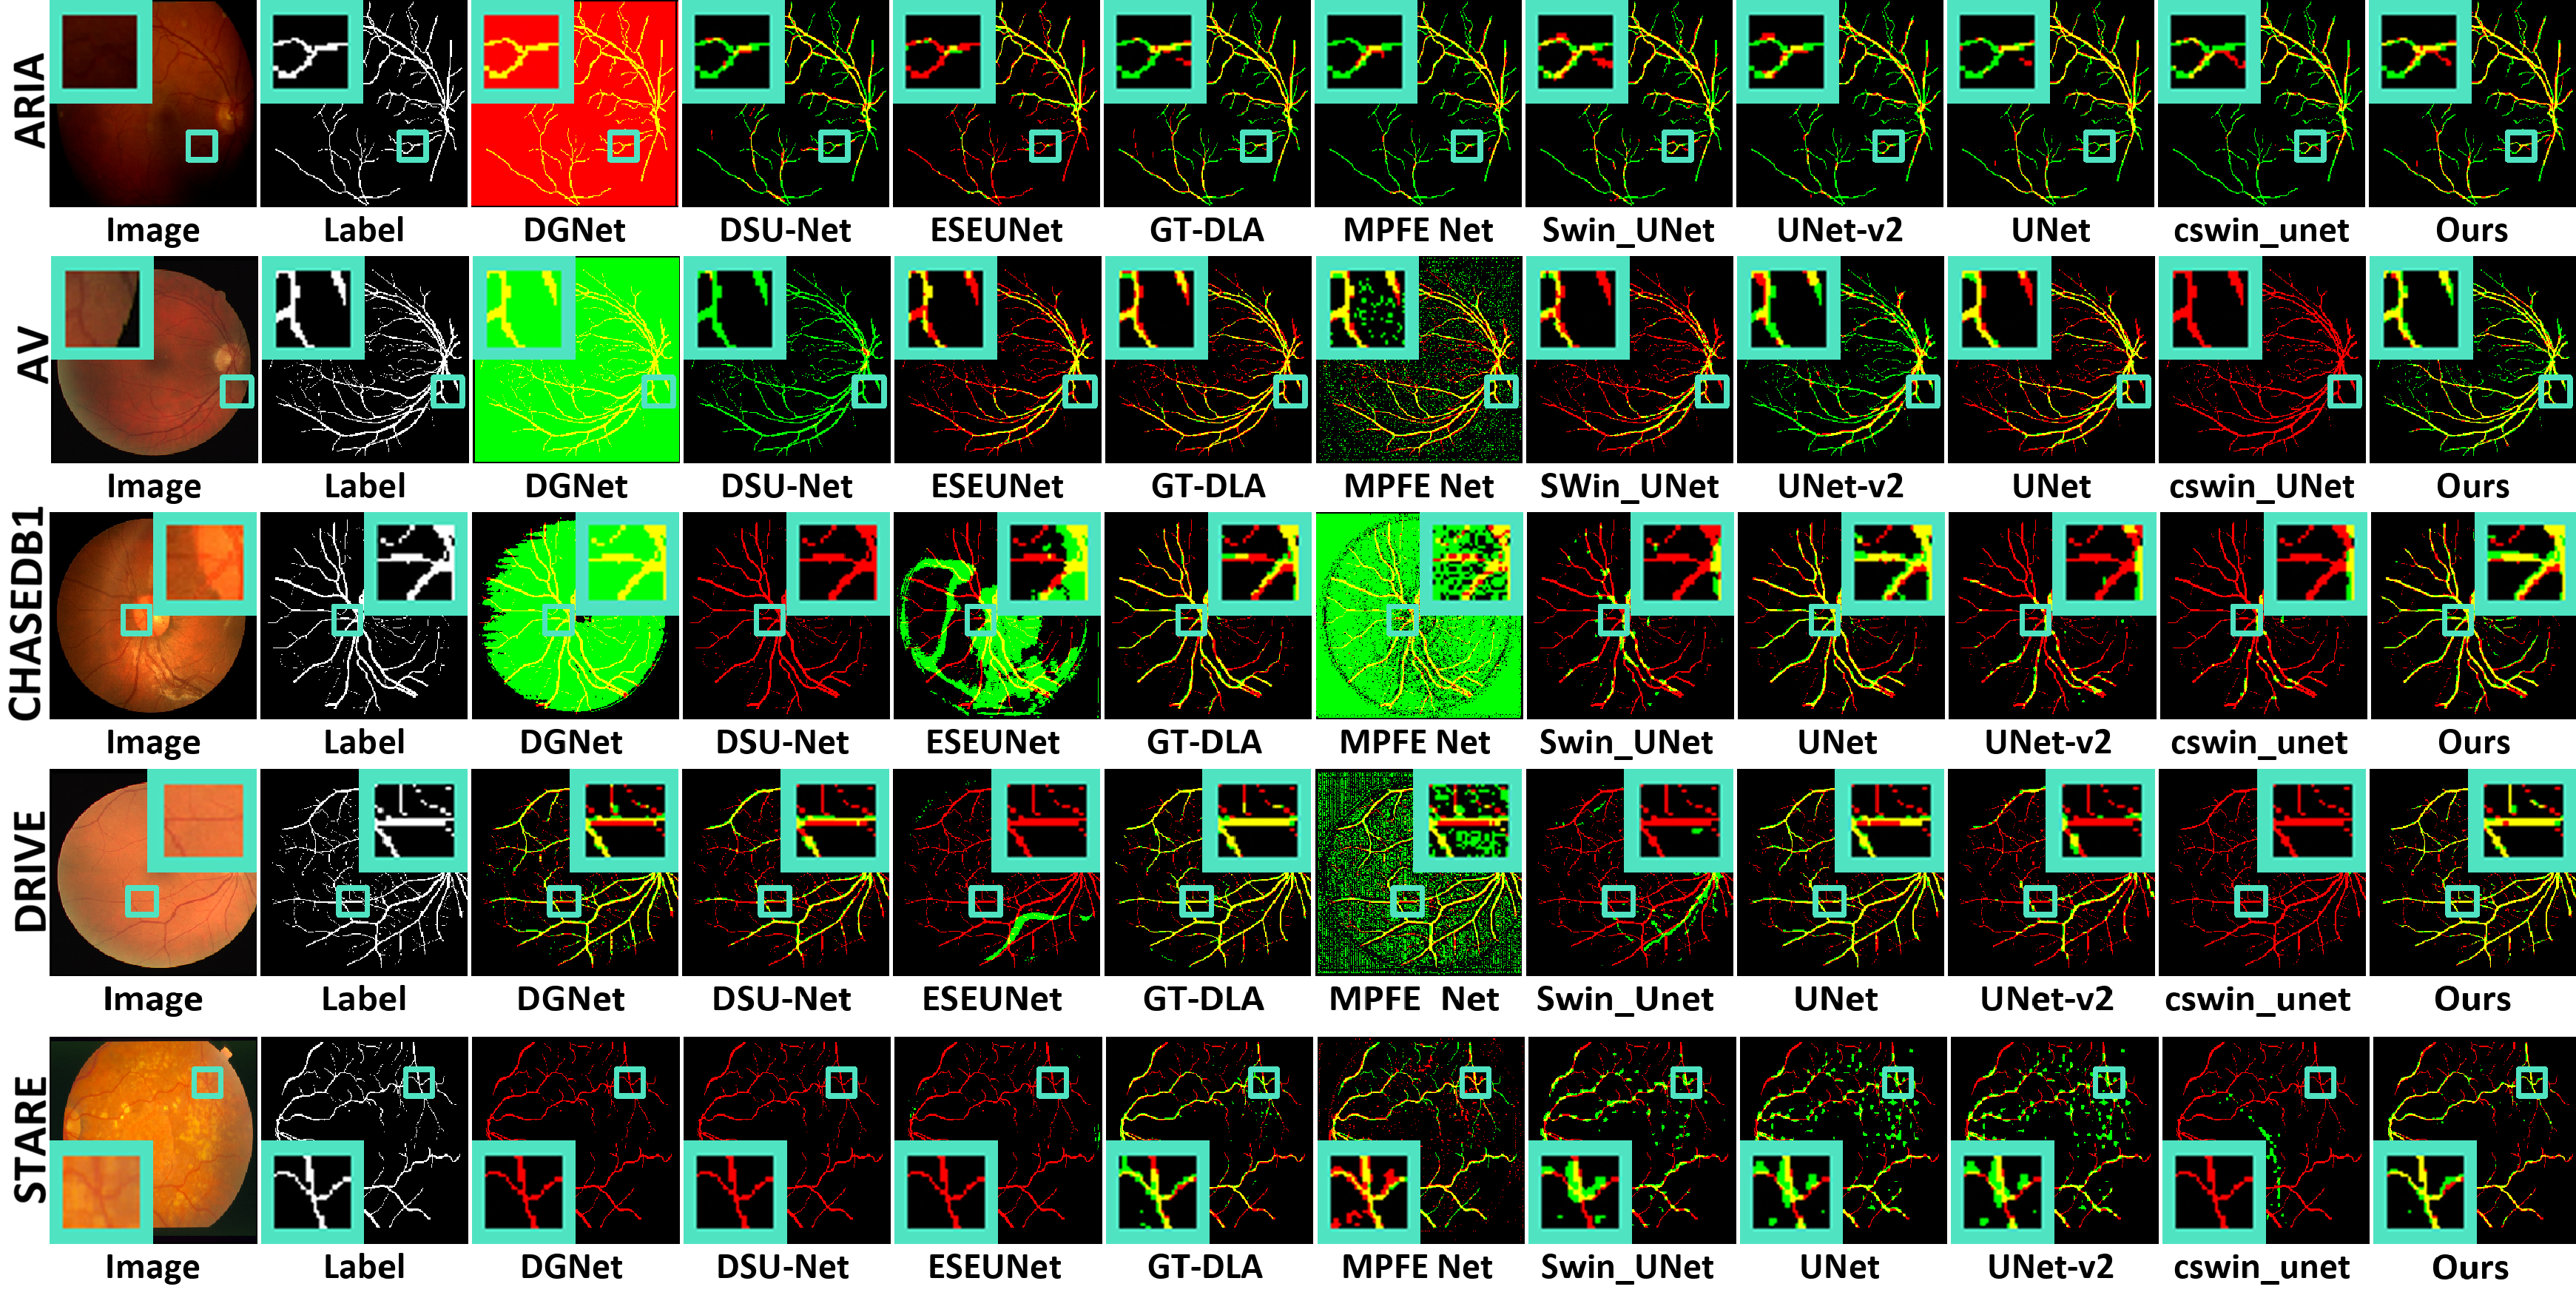
\includegraphics[width=0.90\linewidth]{fig09-qualitative-comparison.png}
    \caption{Qualitative comparison on five retinal vessel segmentation datasets. Each row presents an input image, the corresponding manual label, predictions from the comparison methods, and the EGCS-Net prediction. The cyan boxes identify a local region that is enlarged within each panel for closer inspection.}
    \label{fig:222}
\end{figure}

The marked regions contain vessel terminals, bifurcations, or locally weak responses that expose differences among the predictions.
Several comparison methods omit label-supported vessel segments or produce isolated responses around the selected regions.
The EGCS-Net predictions retain more of the connected structures shown in the manual labels while limiting some of the disconnected background responses visible in the comparison outputs.
These examples provide qualitative context for the Dice, IoU, and precision results in Table~\ref{tab:main_comparison}; they are not treated as causal evidence for an individual module.

\subsection{Cross-Architecture Transfer}

The compatibility of RCE, SGC, and CSP with other segmentation architectures was evaluated using U-Net, TransUNet, and UNet++ as host backbones.
The three modules were integrated into each backbone and evaluated on CHASEDB1, STARE, AV-WIDE, and ARIA while the remaining host architecture was retained.
Figure~\ref{fig:transfer_gains} reports the changes in Dice and IoU relative to the corresponding backbone without the proposed modules.

\begin{figure}[pos=!htbp]
    \centering
    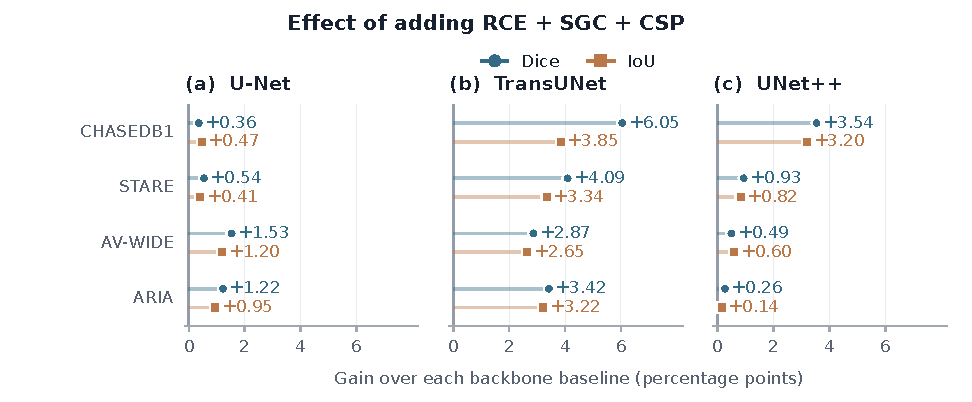
\includegraphics[width=0.82\linewidth]{fig-transfer-backbone-gains.pdf}
    \caption{Cross-architecture transfer of RCE, SGC, and CSP to (a) U-Net, (b) TransUNet, and (c) UNet++ on four retinal vessel segmentation datasets. Blue circles and orange squares denote Dice and IoU gains, respectively, in percentage points. Each gain is the score after integrating all three modules minus the corresponding backbone baseline score. All panels use the same horizontal scale; positive values indicate improved overlap.}
    \label{fig:transfer_gains}
\end{figure}

Integrating the three modules improves Dice and IoU for every evaluated backbone-dataset pair.
TransUNet shows the largest gains on both metrics across the four datasets.
The gains for U-Net and UNet++ are smaller and vary across datasets, with UNet++ showing its largest improvement on CHASEDB1 and only a small change on ARIA.
These results support compatibility with the tested host architectures, while the variation in gains indicates that the benefit depends on the backbone and dataset.

\subsection{Overall Module Ablation}

The overall ablation study evaluates how RCE, SGC, and CSP contribute to EGCS-Net when they are used individually and in combination.
The dual-branch architecture without the three modules serves as the baseline, and all module configurations are compared under the same experimental setting.
Table~\ref{tab:ablation_all} reports Dice and IoU on the five datasets and their averages.

\begin{table}[pos=!htbp]
\centering
\caption{Module-combination ablation study on five retinal vessel segmentation datasets. Check marks indicate the modules included in each configuration. Dice and IoU (\%) are reported for each dataset and as five-dataset averages. The highest and second-highest values in each column are shown in \textbf{bold} and \underline{underlined}, respectively.}
\label{tab:ablation_all}
\scriptsize
\setlength{\tabcolsep}{4pt}
\renewcommand{\arraystretch}{1.08}

\begin{adjustbox}{max width=\textwidth,center}
\begin{tabular}{ccccccccccccccc}
\toprule
\multirow{2}{*}{RCE} &
\multirow{2}{*}{SGC} &
\multirow{2}{*}{CSP}
& \multicolumn{2}{c}{DRIVE}
& \multicolumn{2}{c}{CHASEDB1}
& \multicolumn{2}{c}{STARE}
& \multicolumn{2}{c}{AV-WIDE}
& \multicolumn{2}{c}{ARIA}
& \multicolumn{2}{c}{Average} \\
\cmidrule(lr){4-5}
\cmidrule(lr){6-7}
\cmidrule(lr){8-9}
\cmidrule(lr){10-11}
\cmidrule(lr){12-13}
\cmidrule(lr){14-15}
& & & Dice & IoU & Dice & IoU & Dice & IoU & Dice & IoU & Dice & IoU & Dice & IoU \\
\midrule
$\times$ & $\times$ & $\times$
& \underline{61.26} & \underline{45.62}
& 54.74 & 39.57
& 44.05 & 30.27
& 57.90 & 42.08
& 53.93 & 37.60
& 54.38 & 39.03 \\

$\checkmark$ & $\times$ & $\times$
& 59.49 & 43.54
& 54.13 & 39.35
& 44.97 & 31.04
& 58.91 & 42.90
& 54.67 & 38.21
& 54.43 & 39.01 \\

$\times$ & $\checkmark$ & $\times$
& 57.79 & 42.39
& 53.55 & 38.98
& 45.95 & 32.08
& 56.02 & 40.58
& 52.54 & 36.44
& 53.17 & 38.09 \\

$\times$ & $\times$ & $\checkmark$
& 59.87 & 43.90
& 55.82 & 40.63
& 44.32 & 30.73
& 58.58 & 42.80
& 54.64 & 38.21
& 54.65 & 39.25 \\

$\checkmark$ & $\checkmark$ & $\times$
& 59.98 & 44.51
& 54.55 & 39.69
& 46.18 & 32.16
& 59.50 & 43.83
& 54.54 & 38.15
& 54.95 & 39.67 \\

$\checkmark$ & $\times$ & $\checkmark$
& 59.89 & 43.81
& \underline{56.74} & \underline{41.56}
& \underline{46.47} & \underline{32.37}
& 60.08 & 44.29
& 54.11 & 37.80
& \underline{55.46} & \underline{39.97} \\

$\times$ & $\checkmark$ & $\checkmark$
& 59.50 & 44.16
& 55.72 & 40.60
& 45.66 & 31.52
& \underline{60.26} & \underline{44.37}
& \underline{54.80} & \underline{38.26}
& 55.19 & 39.78 \\
\midrule
$\checkmark$ & $\checkmark$ & $\checkmark$
& \textbf{61.36} & \textbf{45.87}
& \textbf{57.08} & \textbf{42.23}
& \textbf{49.61} & \textbf{34.92}
& \textbf{60.69} & \textbf{45.02}
& \textbf{55.98} & \textbf{39.43}
& \textbf{56.94} & \textbf{41.49} \\
\bottomrule
\end{tabular}
\end{adjustbox}
\end{table}

The complete configuration improves the five-dataset average Dice and IoU by 2.56 and 2.46 percentage points, respectively, relative to the baseline.
Every single-module and two-module configuration remains below the complete model on the two average overlap metrics.
Among the partial configurations, RCE with CSP gives the highest average Dice and IoU, but it remains 1.48 and 1.52 percentage points below the complete model.
The result supports the use of the three modules as complementary parts of the ordered RCE to SGC to CSP processing chain.

\subsection{RCE Ablation Analysis}

The RCE ablation compares four reference configurations: no RCE, a fixed center, a learned center, and a learned center with reliability gating.
Only the reference-center configuration is changed within this comparison.
Table~\ref{tab:rce_ablation} reports the resulting Dice and IoU values.

\begin{table}[pos=!htbp]
\centering
\caption{Ablation of the reference configuration used by RCE. Dice and IoU (\%) are reported on five retinal vessel segmentation datasets. The learned-center configuration with reliability gating corresponds to the complete RCE setting. The highest and second-highest values in each column are shown in \textbf{bold} and \underline{underlined}, respectively.}
\label{tab:rce_ablation}
\scriptsize
\setlength{\tabcolsep}{4pt}
\renewcommand{\arraystretch}{1.08}

\begin{adjustbox}{max width=\textwidth,center}
\begin{tabular}{lcccccccccccc}
\toprule
\multirow{2}{*}{Setting}
& \multicolumn{2}{c}{DRIVE}
& \multicolumn{2}{c}{CHASEDB1}
& \multicolumn{2}{c}{STARE}
& \multicolumn{2}{c}{AV-WIDE}
& \multicolumn{2}{c}{ARIA}
& \multicolumn{2}{c}{Average} \\
\cmidrule(lr){2-3}
\cmidrule(lr){4-5}
\cmidrule(lr){6-7}
\cmidrule(lr){8-9}
\cmidrule(lr){10-11}
\cmidrule(lr){12-13}
& Dice & IoU & Dice & IoU & Dice & IoU & Dice & IoU & Dice & IoU & Dice & IoU \\
\midrule
w/o RCE
& 58.53 & 42.88
& 54.62 & 39.81
& 45.25 & 31.30
& 56.41 & 40.87
& 54.36 & 38.07
& 53.83 & 38.59 \\

Fixed center
& 58.89 & 43.47
& 54.98 & 40.26
& 45.72 & 31.69
& \underline{57.63} & \underline{42.27}
& 55.18 & 38.64
& 54.48 & 39.27 \\

Learned center
& \underline{59.30} & \underline{44.01}
& \underline{56.17} & \underline{41.11}
& \underline{46.81} & \underline{32.68}
& 57.62 & 42.23
& \underline{55.37} & \underline{38.86}
& \underline{55.05} & \underline{39.78} \\

Learned center + reliability gating
& \textbf{61.36} & \textbf{45.87}
& \textbf{57.08} & \textbf{42.23}
& \textbf{49.61} & \textbf{34.92}
& \textbf{60.69} & \textbf{45.02}
& \textbf{55.98} & \textbf{39.43}
& \textbf{56.94} & \textbf{41.49} \\
\bottomrule
\end{tabular}
\end{adjustbox}
\end{table}

The average Dice and IoU increase from 53.83\% and 38.59\% without RCE to 54.48\% and 39.27\% with a fixed center and to 55.05\% and 39.78\% with a learned center.
Adding reliability gating to the learned center produces averages of 56.94\% and 41.49\%.
Relative to the configuration without RCE, the complete RCE setting increases the average Dice and IoU by 3.11 and 2.90 percentage points, respectively.
Within the tested configurations, the result supports estimating the reference from image features and regulating its downstream contribution with the reliability term.

\subsection{SGC Ablation Analysis}

\subsubsection{Sector Organization and Cross-Sector Interaction}

Three configurations isolate the effects of sector-based token organization and multi-head attention (MHA).
Configuration A is the complete SGC design, Configuration B replaces sector tokens with grid tokens, and Configuration C retains sector tokens but removes MHA.
The results are reported in Table~\ref{tab:sgc_attention_comparison}.

\begin{table}[pos=!htbp]
\centering
\caption{Comparison of token organization and interaction strategies in SGC. Configuration A uses sector tokens with MHA, Configuration B uses grid tokens with MHA, and Configuration C uses sector tokens without MHA. Dice and IoU (\%) are reported. The highest and second-highest values in each column are shown in \textbf{bold} and \underline{underlined}, respectively.}
\label{tab:sgc_attention_comparison}
\scriptsize
\setlength{\tabcolsep}{4pt}
\renewcommand{\arraystretch}{1.08}

\begin{adjustbox}{max width=\textwidth,center}
\begin{tabular}{lcccccccccccc}
\toprule
\multirow{2}{*}{Setting}
& \multicolumn{2}{c}{DRIVE}
& \multicolumn{2}{c}{CHASEDB1}
& \multicolumn{2}{c}{STARE}
& \multicolumn{2}{c}{AV-WIDE}
& \multicolumn{2}{c}{ARIA}
& \multicolumn{2}{c}{Average} \\
\cmidrule(lr){2-3}
\cmidrule(lr){4-5}
\cmidrule(lr){6-7}
\cmidrule(lr){8-9}
\cmidrule(lr){10-11}
\cmidrule(lr){12-13}
& Dice & IoU & Dice & IoU & Dice & IoU & Dice & IoU & Dice & IoU & Dice & IoU \\
\midrule
A: Sector-token + MHA
& \textbf{61.36} & \textbf{45.87}
& \textbf{57.08} & \textbf{42.23}
& \textbf{49.61} & \textbf{34.92}
& \textbf{60.69} & \textbf{45.02}
& \textbf{55.98} & \underline{39.43}
& \textbf{56.94} & \textbf{41.49} \\

B: Grid-token + MHA
& 59.34 & 43.91
& \underline{55.60} & \underline{40.94}
& 47.87 & 33.81
& 60.16 & \underline{44.81}
& \underline{55.97} & \textbf{39.52}
& 55.79 & \underline{40.60} \\

C: Sector-token w/o MHA
& \underline{59.88} & \underline{44.21}
& 55.19 & 40.06
& \underline{48.59} & \underline{34.00}
& \underline{60.35} & 44.71
& 55.42 & 38.85
& \underline{55.88} & 40.37 \\
\bottomrule
\end{tabular}
\end{adjustbox}
\end{table}

Configuration A reaches average Dice and IoU values of 56.94\% and 41.49\%, compared with 55.79\% and 40.60\% for the grid-token configuration.
Removing MHA while retaining sector tokens gives averages of 55.88\% and 40.37\%.
The corresponding reductions support both the center-conditioned sector organization and cross-sector interaction in the tested SGC design.

\subsubsection{Internal Design and Placement}

Figure~\ref{fig:sandian} summarizes the average Dice and IoU obtained when changing the sector count \(K\), ring construction, confidence and reliability terms, and SGC placement.

\begin{figure}[pos=!htbp]
    \centering
    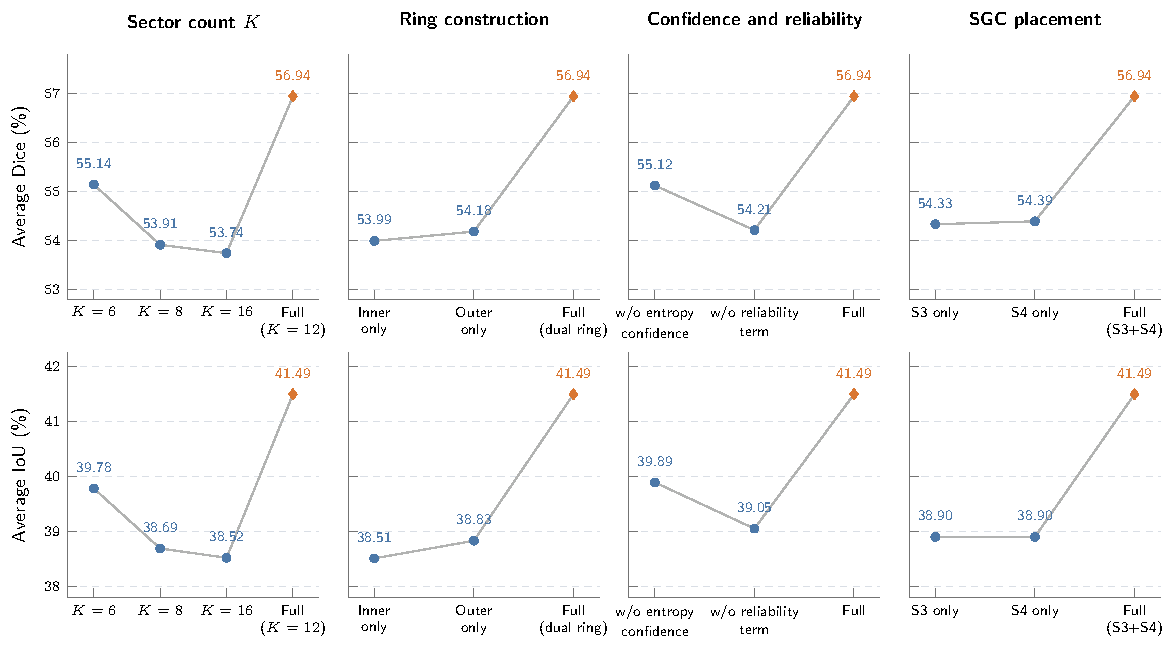
\includegraphics[width=\linewidth]{fig12-sgc-design-ablation.pdf}
    \caption{Average Dice and IoU for the internal SGC design comparisons across five datasets. The upper and lower rows report Dice and IoU, respectively. The four columns compare the sector count \(K\), ring construction, confidence and reliability terms, and SGC placement. Each panel contrasts the tested alternative settings with the complete configuration.}
    \label{fig:sandian}
\end{figure}

For the sector-count comparison, \(K=12\) gives higher average Dice and IoU than \(K=6\), \(K=8\), and \(K=16\).
The dual-ring construction also exceeds the inner-only and outer-only alternatives on both overlap metrics.
Removing either entropy-based confidence or the reliability term lowers the two averages.
The placement comparison follows the same pattern: applying SGC at S3 and S4 gives higher average Dice and IoU than applying it at either stage alone.
These comparisons define the selected SGC configuration without treating the ablation differences as statistical or causal proof.

\subsection{CSP Ablation Analysis}

\subsubsection{Component Analysis}

The component ablation removes one listed CSP component at a time while retaining the remaining settings.
Figure~\ref{fig:zhuzhuang} summarizes the component, offset-set, and deployment-stage comparisons for each dataset and their average.

% User-approved layout insertion; plotted data await user correction to manuscript values.
\begin{figure}[pos=!htbp]
    \centering
    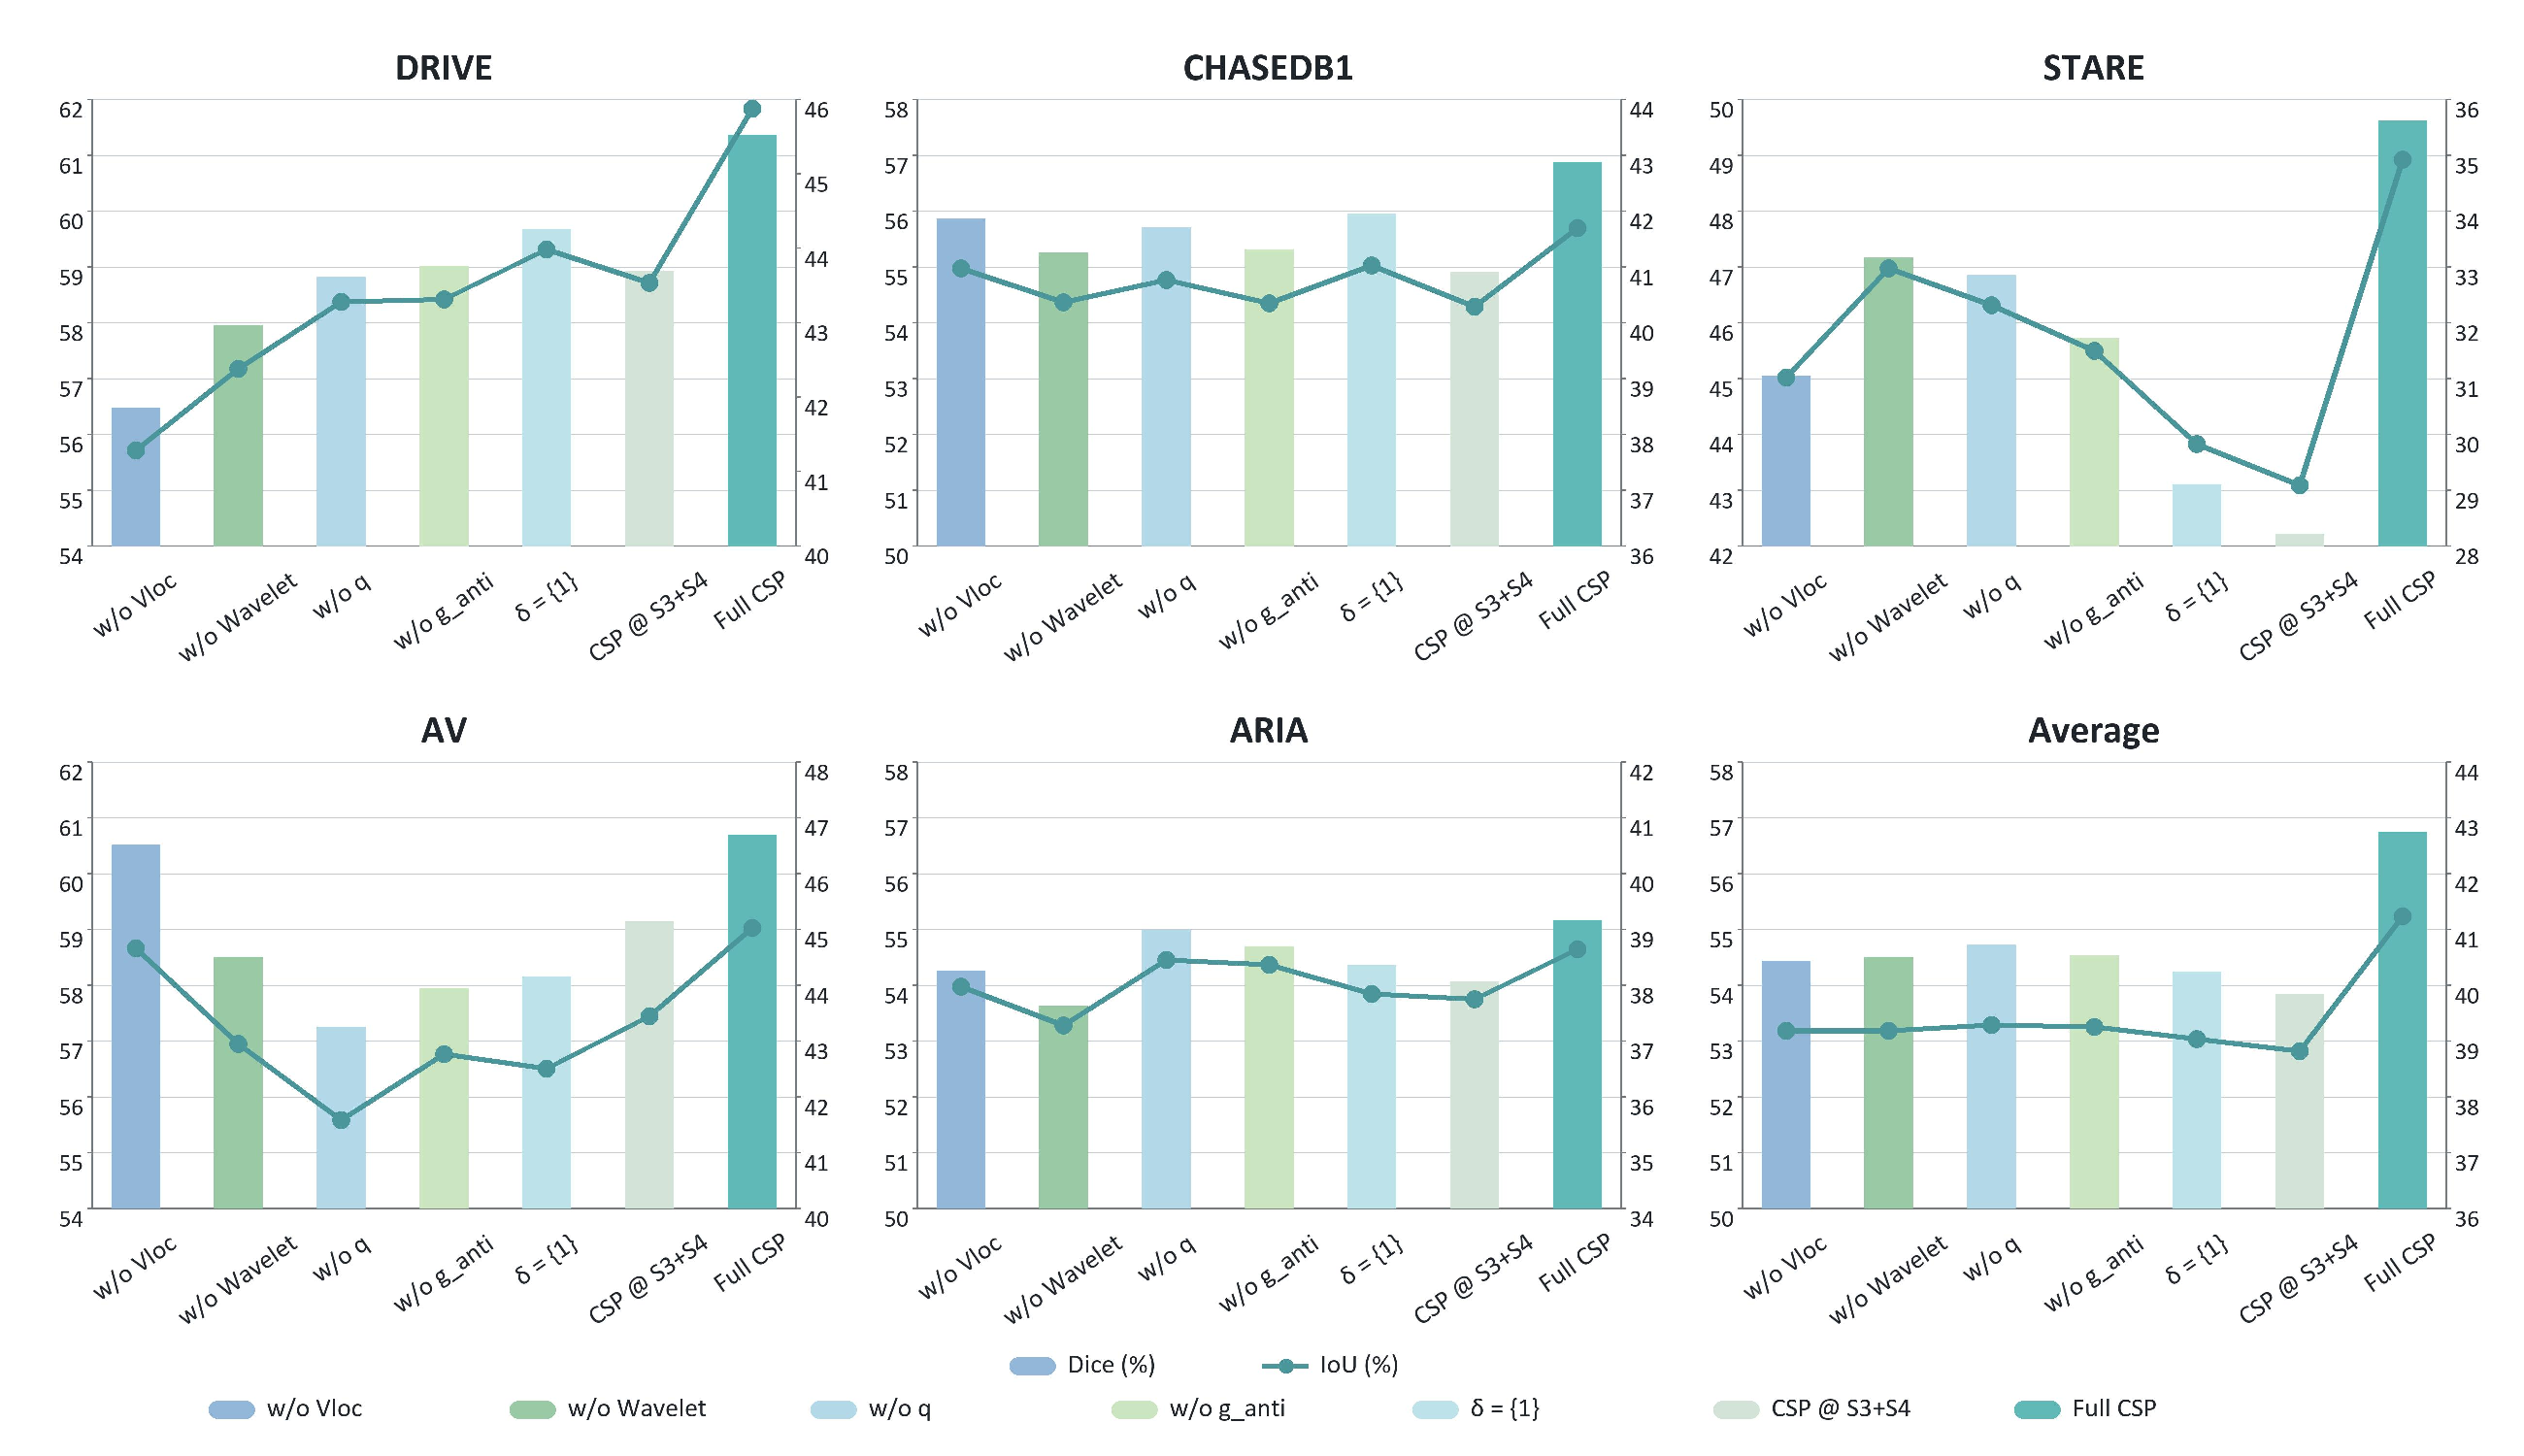
\includegraphics[width=\linewidth]{fig-csp-ablation-user.pdf}
    \caption{CSP ablation across five retinal vessel segmentation datasets and their average. Bars report Dice (\%, left axis), and the line reports IoU (\%, right axis). AV denotes AV-WIDE. The first four settings remove one CSP component at a time; the remaining settings compare the offset set \(\delta=\{1\}\), deployment at S3 and S4, and Full CSP with \(\delta=\{1,2,4\}\) at S3. Axis ranges vary across panels.}
    \label{fig:zhuzhuang}
\end{figure}

The complete CSP configuration obtains average Dice and IoU values of 56.94\% and 41.49\%, respectively.
Removing any one of the four listed components lowers both averages.
The average Dice reductions range from 2.22 to 2.51 percentage points, and the IoU reductions range from 2.21 to 2.31 percentage points.
These results support retaining the four components in the evaluated CSP configuration.

Figure~\ref{fig:no_CSP} provides qualitative examples corresponding to the CSP ablation.

\begin{figure}[pos=!htbp]
    \centering
    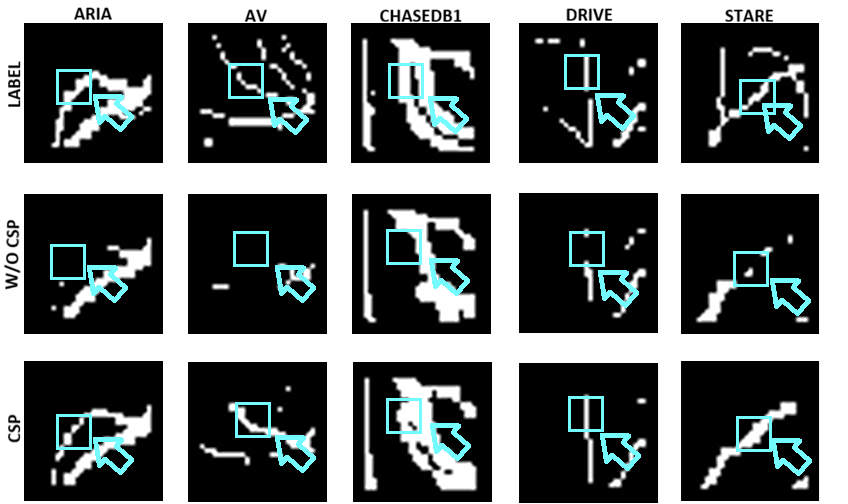
\includegraphics[width=0.86\linewidth]{fig11-csp-ablation-visualization.png}
    \caption{Qualitative CSP ablation examples on ARIA, AV-WIDE, CHASEDB1, DRIVE, and STARE. The rows show the manual labels, predictions without CSP, and predictions with CSP, respectively. Cyan boxes and arrows identify local regions used to compare vessel continuity and isolated responses.}
    \label{fig:no_CSP}
\end{figure}

Within the highlighted regions, predictions without CSP contain missing vessel segments or isolated responses, whereas the predictions with CSP retain more of the local structure shown in the corresponding labels.
The examples are consistent with the component-level differences in Figure~\ref{fig:zhuzhuang}, but they do not isolate the effect of an individual CSP subcomponent.

\subsubsection{Offset Set and Deployment Stage}

Figure~\ref{fig:zhuzhuang} also compares the SCB offset set and CSP deployment stage.
The complete configuration uses \(\delta=\{1,2,4\}\) and applies CSP at S3.



Using only \(\delta=\{1\}\) gives average Dice and IoU values of 54.24\% and 39.03\%, which are 2.70 and 2.46 percentage points below the complete configuration.
Applying CSP at both S3 and S4 gives averages of 53.84\% and 38.81\%, corresponding to reductions of 3.10 and 2.68 percentage points.
Within the evaluated settings, the selected offset set and S3 deployment provide the highest average Dice and IoU.

\section{Discussion}

Figure~\ref{fig:can} summarizes the computational profile used to assess the efficiency cost of explicit geometric conditioning.

\begin{figure}[pos=!htbp]
    \centering
    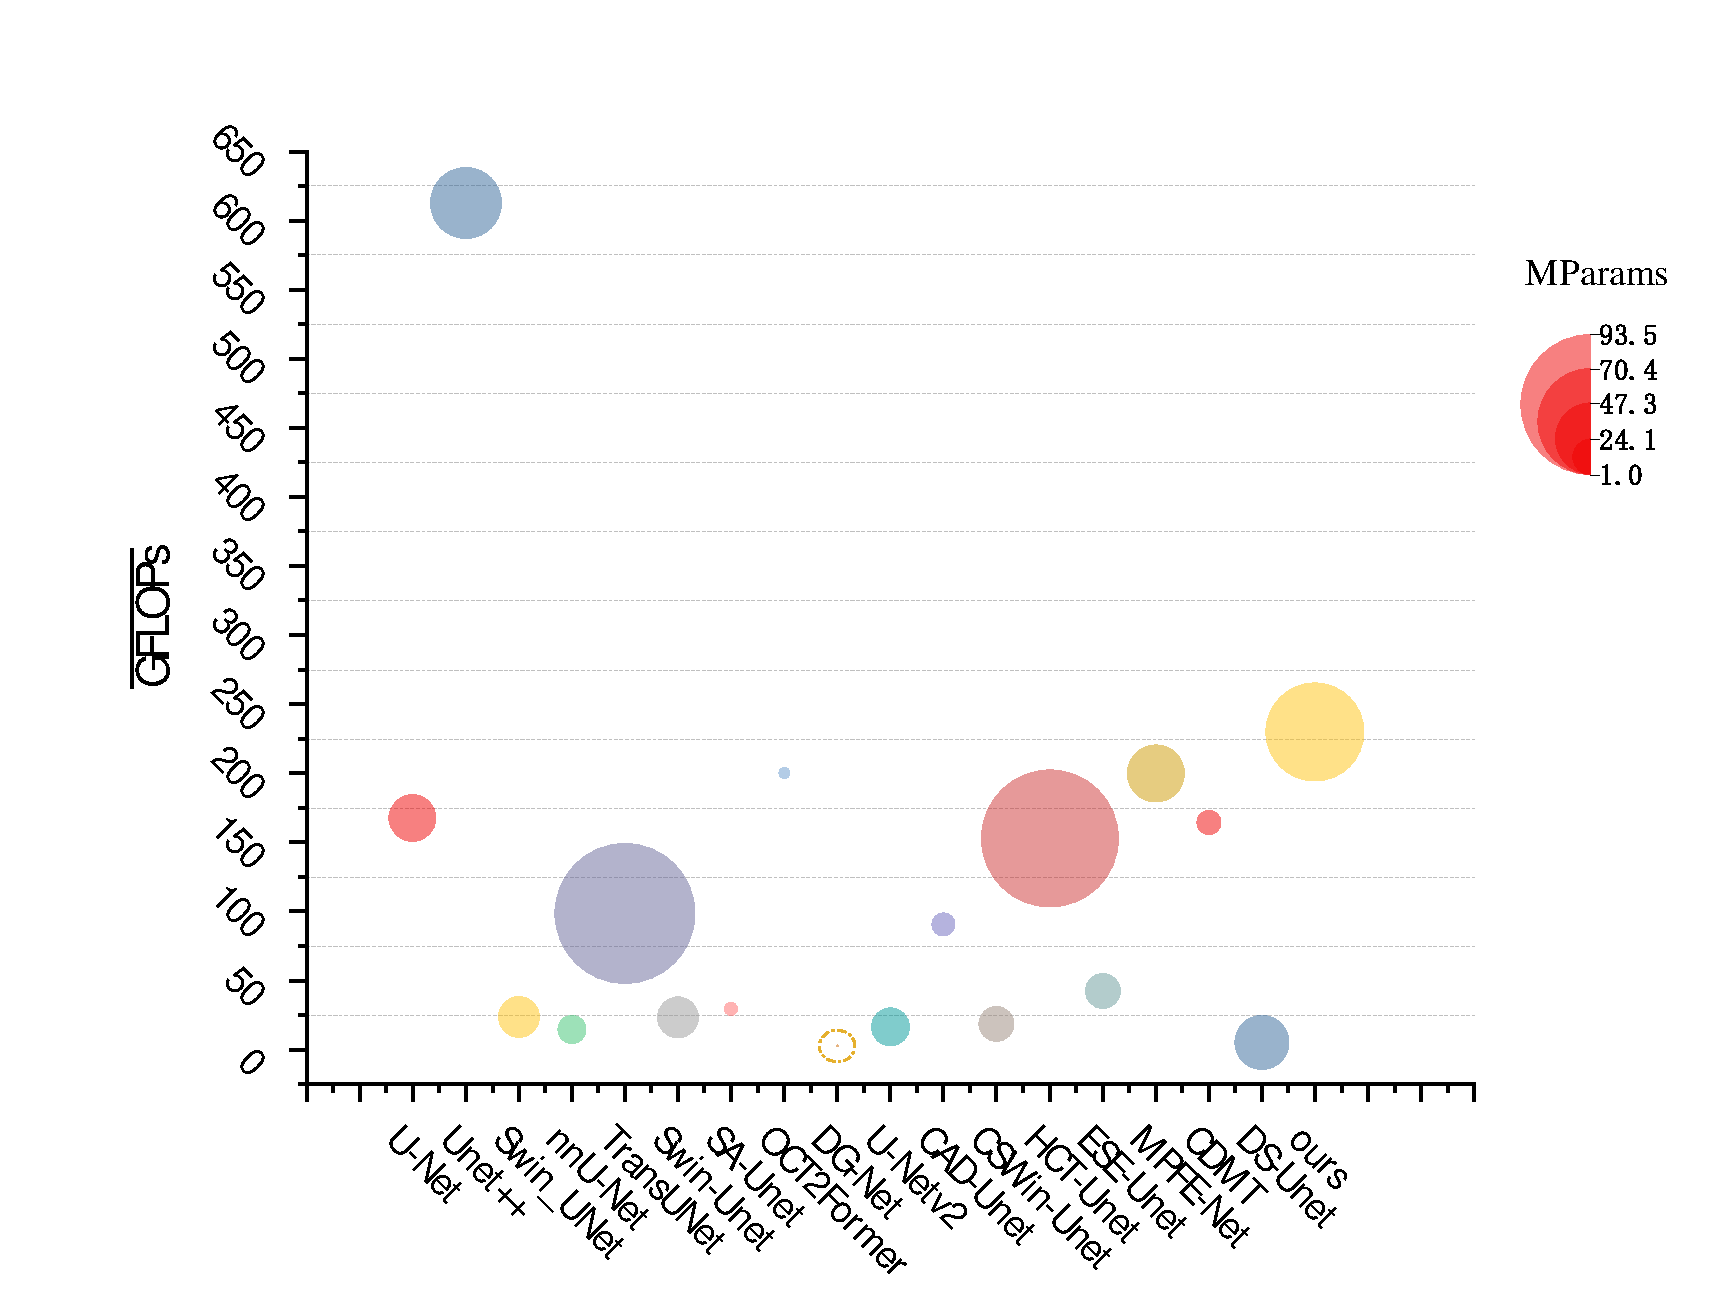
\includegraphics[width=0.82\linewidth]{fig-computational-cost-user.pdf}
    \caption{Computational cost of the compared segmentation models. The vertical axis reports GFLOPs, and bubble size represents the number of parameters in millions (MParams). The horizontal axis identifies each model; ``ours'' denotes EGCS-Net.}
    \label{fig:can}
\end{figure}

EGCS-Net requires 230.03 GFLOPs and contains 65.23 M parameters.
All compared models were profiled at the same input resolution using the same computational-cost estimation protocol and parameter-counting convention, so the values in Figure~\ref{fig:can} are directly comparable within this analysis.
The measured cost reflects the complete dual-branch coarse-to-fine framework and the ordered RCE, SGC, and CSP processing chain.
The present profile reports total model cost rather than component-specific overhead.
It therefore defines a concrete trade-off between explicit geometric organization and computational efficiency without implying suitability for a particular deployment setting.
A useful next step is to report module-level FLOPs, memory use, and inference latency under the same protocol, then examine whether computation can be shared across the two branches or reduced within sector interaction and high-resolution skip purification while preserving the observed segmentation performance.

RCE provides an image-dependent structural reference without requiring an additional anatomical annotation target.
Its reliability term regulates the downstream contribution of the learned reference state when the center response is diffuse.
Accordingly, the reference is treated as a learned geometric state rather than an anatomical localization result.
The experiments on AV-WIDE, ARIA, DRIVE, CHASEDB1, and STARE, together with transfer experiments on U-Net, TransUNet, and UNet++, support the use of the RCE to SGC to CSP mechanism within the evaluated datasets and host architectures.
They do not separately quantify sensitivity to controlled center perturbations or changes in imaging conditions.
Further evaluation can therefore combine controlled perturbations of the center state with data acquired under different imaging systems and acquisition protocols.
Such experiments would identify the conditions under which the learned reference remains informative without extending the present conclusions beyond the available evidence.

The reported evaluation combines Dice, IoU, sensitivity, specificity, precision, AUC, and accuracy with qualitative comparisons.
These metrics characterize region overlap and pixelwise discrimination, while the qualitative examples illustrate vessel continuity, terminal recovery, and isolated background responses.
Neither form of evidence directly quantifies centerline continuity or branch preservation across the complete vascular tree.
Future studies should therefore complement the current protocol with structure-aware measures such as clDice~\cite{shit2021cldice} and connectivity-based criteria.
Reporting these measures alongside the existing metrics would distinguish improvements in regional segmentation from improvements in structural integrity and would align the evaluation more closely with the geometry-conditioned structure-recovery objective of EGCS-Net.
This extension is an evaluation priority rather than a claim about performance that has not yet been measured.

\section{Conclusion}

EGCS-Net formulates retinal vessel segmentation as geometry-conditioned structure recovery within a dual-branch coarse-to-fine framework.
The structure-prior branch estimates global vessel structure and supplies geometric conditions, while the detail-refinement branch reconstructs the final high-resolution prediction through cascaded and same-scale feature injection.
Within this framework, RCE provides a learned reference state and its reliability, SGC organizes vessel features through angular and radial relationships, and CSP controls the high-resolution skip information used for final reconstruction.
Their ordered connection addresses three limitations of conventional Cartesian dense prediction: the absence of a computable structural reference, the need to represent locally consistent but spatially varying vessel directions, and the propagation of texture noise or pseudo-boundary responses through shallow skip features.
EGCS-Net therefore connects structural anchoring, geometry-aware feature organization, and controlled detail reconstruction in a single processing chain.

Across AV-WIDE, ARIA, DRIVE, CHASEDB1, and STARE, EGCS-Net obtains the highest Dice and IoU among the evaluated methods on each dataset, with five-dataset averages of 56.94\% and 41.49\%, respectively.
Cross-architecture transfer experiments show that integrating RCE, SGC, and CSP improves Dice and IoU for the tested U-Net, TransUNet, and UNet++ backbones, while the module and internal ablations support the contribution of the evaluated components and placement choices.
Together, these results support explicit geometric conditioning for retinal vessel structure recovery within the reported datasets, comparison set, and host architectures.
Future work will focus on reducing the computational cost of the framework and extending evaluation through controlled perturbations of the learned center state and structure-aware measures of vascular continuity.

\section*{Acknowledgments}
This research was supported by Sichuan Science and Technology Program (2026NSFSC1484). In addition, the
computational platform for this study was supported by the National Supercomputing Center in Chengdu-Chengdu
University Branch. We also thank Xueheng Li for supporting the technical work of this paper.

%% Loading bibliography style file
\bibliographystyle{unsrt}

%% Loading bibliography database
\bibliography{references/references}

%% Biography (commented out)
%\bio{}
% Here goes the biography details.
%\endbio

%\bio{pic1}
% Here goes the biography details.
%\endbio

\end{document}
